%Vorlage
\documentclass[12pt,a4paper]{scrartcl}
\usepackage[english]{babel} %Für die indirekte Angabe von Umlauten. Es müssen dann Umlaute wie folgt im Code angegeben werden: "a "o "u "s.

\usepackage[utf8]{inputenc}
%Math
\usepackage{amsmath, amsthm, amssymb}
\usepackage{braket}
\newcommand{\tens}[1]{% https://tex.stackexchange.com/questions/171788/always-have-the-ring-of-the-tensor-product-below-the-otimes -> Tensor Product
  \mathbin{\mathop{\otimes}\displaylimits_{#1}}%
}
%Page numbers
\usepackage{enumerate}
%Graphics
\usepackage{graphicx}
\usepackage{array}% http://ctan.org/pkg/array
\usepackage{floatrow}
\graphicspath{{./images/}}
%Quantum circuits http://mirrors.ibiblio.org/CTAN/graphics/pgf/contrib/quantikz/quantikz.pdf
\usepackage{tikz}
\usetikzlibrary{quantikz}
\usepackage{lscape}
\usepackage{setspace}
\onehalfspacing
\usepackage{wrapfig}
\usepackage{hyperref}% für die Einbettung von Hyperlinks
\def\UrlBreaks{\do\/\do-}
\usepackage{multirow}
\usepackage{csquotes} %Quotations
%Code
\usepackage{pythonhighlight}


% Margins
%\usepackage{geometry} % Document Margins
%\setlength{\topmargin}{0cm}
%\setlength{\parindent}{5mm}
%\setlength{\parskip}{2mm}
%\setlength{\evensidemargin}{0mm}
%\setlength{\oddsidemargin}{0cm}
\pagestyle{headings}



\begin{document}
\thispagestyle{empty}
\vspace*{-3cm}
\begin{center}
\large \textsc{Bern University of Applied Sciences}
\vspace{0.5cm}
\hrule
\vspace{4.5cm}
{\Large \textsc{Project II - BTI7302}}\\
{\large HS 2020/21}\\
\vspace{1cm}
{\Large \bfseries
Computer vision methods for detection of early retinal thickness changes in myopic Asian school children}\\
\vspace*{1cm}
{\large Tutor:  Prof. Dr. Tiziano Ronchetti}
\end{center}
\vspace*{1cm}

\begin{abstract}
\textbf{Abstract: }Retinal layers thickness measurement offers physicians a reliable method for diagnose and treatment of ocular and other diseases. The computerized implementation of this technique involves the utilisation of computer vision algorithms in order to detect and measure retinal layers from OCT scans. In this report, the authors explore these algorithms and implement the techniques in order to obtain a reliable set of algorithmically generated annotations in order to evaluate the application of machine learning for detecting retinal layers and accurately identifying thickness measurement changes with minimal human intervention. \\
\textbf{Keywords: } Ophthalmology, Retinal Layers, Machine Learning, Computer Vision, Data Analysis
\end{abstract}

\vspace{2cm}
\hspace*{5.2cm}
\parbox{8.2cm}

\begin{tabular}{ll}

Submitted by: & Emeline Liebeherr\\
& Rayner Oswaldo Däppen\\

Submission deadline: & Friday, January 30th, 2021


\end{tabular}

\newpage
\pagenumbering{Roman}
\tableofcontents

\newpage
\pagenumbering{arabic}
%Und nun kommen wir zur Arbeit und fangen an die Seiten mit Arabischen Zahlen zu zählen

\section{Introduction}\label{s:introduction}
The main objective of this paper is to provide an implementation of the most common algorithmic methods used in the field of computer vision for segmenting retinal inner layers obtained from OCT scans in order to produce a reliable set of annotations that can be used in a future work for developing a machine learning model that can accurately detect retinal thickness changes and provide physicians with reliable and factual information that can help in the diagnosis of several pathologies associated to changes in the retinal structure. \\

The relevance of this project lies on the documentation and explanation of the most frequent methods used for measuring retinal thickness from an algorithmic perspective in order to provide engineers with an easy to use guide for extracting features from OCT B-scans. The report is structured as follows. Section 2 presents an introduction to the medical background needed in order to understand the retinal structure, functions and the importance of retinal layer thickness measurement. Section 3 will offer an overview of the most common techniques used in the industry for carrying out retinal layer segmentation from OCT scans. Section 4 will offer the implementation and results of the methods discussed. Finally, section 5 and 6 will respectively offer a conclusion and an overview of the future work to be carried out by the authors. \\

\section{Medical Background}\label{s:medical_background}

The retina is a layer of tissue situated in the periphery of the ocular globe. As a part of the central nervous system, the retina \textit{converts the graded electrical activity of photoreceptors into action potentials that travel to the brain via axons in the optic nerve.}\cite{purves2001} In other terms, it converts light into electric signals that are sent directly to the brain and are interpreted as images. \\

Measuring thickness changes in the retina enable physicians to detect the evolution of certain diseases like Diabetes \cite{Jiang2018}, Alzheimer, Glaucoma and other neurodegenerative diseases \cite{DENHAAN2017162}. For example, in the case of Alzheimer is has been detected in (den Haan et al, 2017) that both measuring methods, Mean Peripapillary Retinal Nerve Fiber Layer (RNFL) and macular thickness show a consistent retinal thinness for diagnosed patients when compared to healthy individuals \cite{DENHAAN2017162}.\\

The process of measuring retinal thickness involves taking a cross sectional scan of the retina and anterior segment, known as Optical Coherence Tomography (OCT). Ocular Bidimensional OCT is a standard, non-invasive procedure in the field of ophthalmology and consist on a micrometer resolution scan of a 2D eye section obtained by emitting low coherence light waves which allow high resolution longitudinal imaging of the corneal, retinal and chroroidal structures \cite{Ronchetti2019statistic}. Locating the retina within a Bidimensional OCT scan (B-Scan) involves the detection of the retina's two boundaries, the Inner Limiting Membrane (ILM) and the Bruchs Membrane (BM). On one side, the ILM serves as a barrier between the retina and the vitreous body \cite{MACNAIR2015343} while the BM divides the retina from the choroid \cite{BOOIJ20101}. The retinal thickness is defined as the average of all Euclidean/vertical distance in the $z$ axis direction between the ILM and BM boundaries \cite{Ronchetti2019statistic}. Another approach to measuring thickness is to define 5 symmetrical regions with respect to the vertical direction, we will name this regions A (subfoveal), B (parafoveal) and C (perifoveal), the thickness values for such regions are provided in the form of the mean of all height differences within a particular section A, B or C respectively \cite{Ronchetti2019statistic} (See Figure \ref{fig:final_rendering}). 

\section{Technical Background}\label{TechBack}

There are several approaches for detecting retinal boundaries, among them we can cite pixel intensity variations, texture analysis and graph based search segmentation techniques all obtained from OCT scans. Pixel intensity variations are often used to calculate the total retinal thickness \cite{Alonso-Caneiro2013}, the method involves a series of computer graphic processing steps where each pixel of the image is compared to a threshold chosen according to the color intensity of the pixels that contain the information about the location of the boundary \cite{Fabritius:09}. In the case of the ILM, it can be extracted easily because the Lens pixels in the OCT scans are mostly black, while the membrane's pixels are mostly white. Therefore, taking the image from the top left corner, one can run a search algorithm that finds the first white pixel \footnote{The first pixel that is over the threshold} from top to bottom and return its position. Running this same algorithm across the $x$ axis will give us an array of pixels that can be smoothed by using cubic-spline interpolations that corresponds to the Internal Limiting Membrane (ILM). The process for extracting the Bruch's Membrane's (BM) inner-most layer is the same, since the sclera presents opaque pixels that can be omitted by the algorithm, the process would start from the bottom left corner and runs the algorithm from bottom to top searching white pixels until it reaches the Bruch's Membrane.      
\section{Results}
- Describe the data set
In this section it will be described how the algorithmic solution to detect ILM and BM from an OCT scan image was implemented. 
After testing different methods for extracting shapes or lines, it became clear that for such an accurate job it is necessary to pre-process the images in a different way than the bare implementation of the classic solutions offered. 
\subsection{ILM Extraction}\label{ILM_Extraction}
The first pre-processing step is to obtain a less nuanced image. As an OCT scan is a variation of grey and the shapes are not always accurate it is therefore more advantageous to work on a black and white image. \\
In order to achieve this result, it is necessary to load the image from the OCT scan into a 2D table (each colour value of a pixel in the image is stored in the table), then run through it pixel by pixel. When a pixel has a value greater than a certain threshold, in this case "25", i.e. a dark grey shade of RGB code (25, 25, 25), that pixel is set to an RGB value (255,255,255), i.e. white, and the rest of the pixels to black. This ensures that only the lightest pixels of the scan are kept. 
\begin{python}
#COL
for j in range(768):
  #LIN
  for i in range(500):
    if imarray[i][j] < 25:
      imarray[i][j] = 0
    else :
      imarray[i][j] = 255
\end{python}

The result here is therefore an extraction of the brightest parts to produce a black and white image :

\begin{figure}[H]
    \centering
    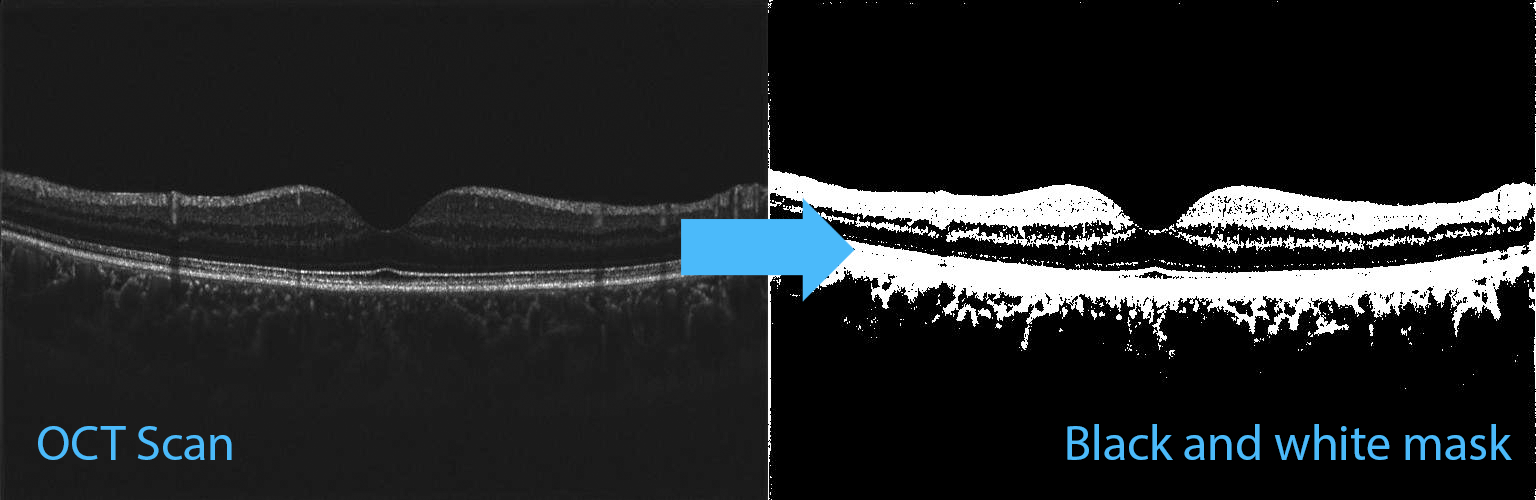
\includegraphics[width=1\textwidth]{./images/OCT_to_BW.png}
    \caption{OCT scan before and after black and white mask processing}
    \label{fig:oct_befor_after}
\end{figure}
As can be seen in Figure \ref{fig:oct_befor_after}: the lens section of the image is completely black. By simply browsing the table containing the new black and white image from top to bottom on each pixel column and extracting only the first white pixel encountered, the following image is obtained: 

\begin{figure}[H]
    \centering
    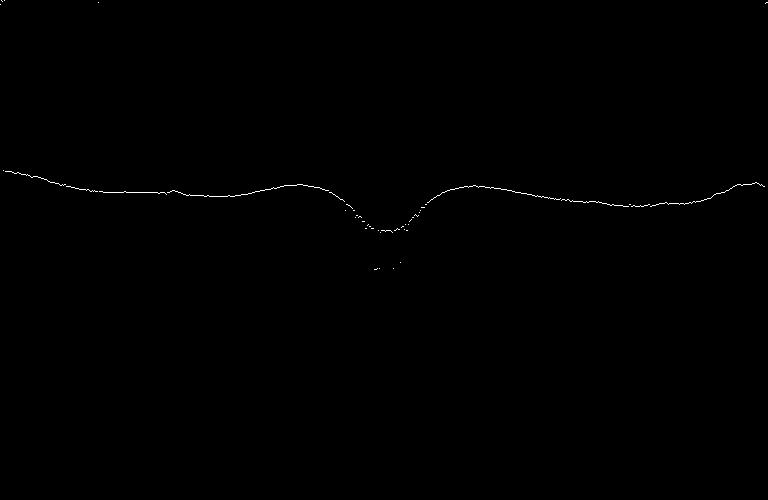
\includegraphics[width=1\textwidth]{./images/ILM_pixel_line_Extracted.jpeg}
    \caption{ILM line pixel extracted}
    \label{fig:ILM_pixel_line}
\end{figure}
At this stage the ILM is roughly extracted because it can be seen that at the place where the scan was darkest, as in the middle, there are still wrong values due to the bad contrast of the scan. The next step is therefore to eliminate the extreme values.
For this purpose, statistics are used to eliminate values that exceed $n$ standard deviations from the mean. This method has been proposed by "transcranial" on Stackoverflow \cite{stackoverflow:transcranial} and translated as follows: 

\begin{quote}
X the y-coordinate of each white pixel.
If for a given x, the absolute value of x minus the average of all x's is smaller than the standard deviation multiplied by n = 1,
So it's an extreme value.
\end{quote}


This allows us to replace them by their neighbouring pixels for values that are too extreme. 

\begin{python}
n = 1
output_ilm = np.zeros(IMG_WIDTH, dtype=object)

for i in range(ilm_array.size):
  if abs(ilm_array[i] - np.mean(ilm_array)) < np.std(ilm_array) * n :
    output_ilm[i]=IMG_HEIGHT -ilm_array[i]
  elif i < 255 :
   #Delete extreme values for extremities (if a extreme value is part of the 10 first of 10 last value, it is set with values next to them)
   j = i
   while abs(ilm_array[j] - np.mean(ilm_array)) > np.std(ilm_array) * n :
     j+=1
   output_ilm[i] = IMG_HEIGHT -ilm_array[j]
  elif i > ilm_array.size - 255 :
    while abs(ilm_array[j] - np.mean(ilm_array)) > np.std(ilm_array) * n :
     j-=1
    output_ilm[i] = IMG_HEIGHT -ilm_array[j]
  else:
    output_ilm[i]=IMG_HEIGHT -ilm_array[i]

\end{python}

Unfortunately, sometimes there is too much "noise" (as the scans are a slightly blurry) in the OCT scan image resulting it a lot of white pixel at the top of the image, introducing errors in the standard deviation which makes it impossible to identify the ILM curve. The solution in this case is to replace all pixels above the height 480 (top pixels) by their neighbouring one if they are brighter than the the standard deviation:
\begin{python}
for i in range(output_ilm.size):
  if output_ilm[i] >= IMG_HEIGHT-20:
    j = i
    while abs(ilm_array[j] - np.mean(ilm_array)) > np.std(ilm_array) * n :
      j+=1
      output_ilm[i] = IMG_HEIGHT -ilm_array[j]
\end{python}

As a result, the ILM is precise enough to apply a smoothing function in order to eliminate the last extreme values and smooth the line to fit the membrane. For this purpose the source code of get\_natural\_cubic\_spline\_model \cite{stackoverflow:np8}
has been used to apply a cubic natural spline model. This allows the ILM curve obtained to be smoothed in a more natural and therefore more accurate way. However, the biggest advantage of this code is that it allows the softness of the natural cubic spline to be controlled. In this way it is possible to manually adapt the ILM rendering for each OCT scan. 

\begin{python}
model_18 = get_natural_cubic_spline_model(x, y, minval=min(x), maxval=max(x), n_knots=18)
y_est_18 = model_18.predict(x)
plt.plot(x*micrometerConversion, y_est_18*micrometerConversion,'r', linewidth=1, marker=',', label='n_knots = 18')
\end{python}

The final image gives an ILM with a fairly good accuracy: 
\begin{figure}[H]
    \centering
    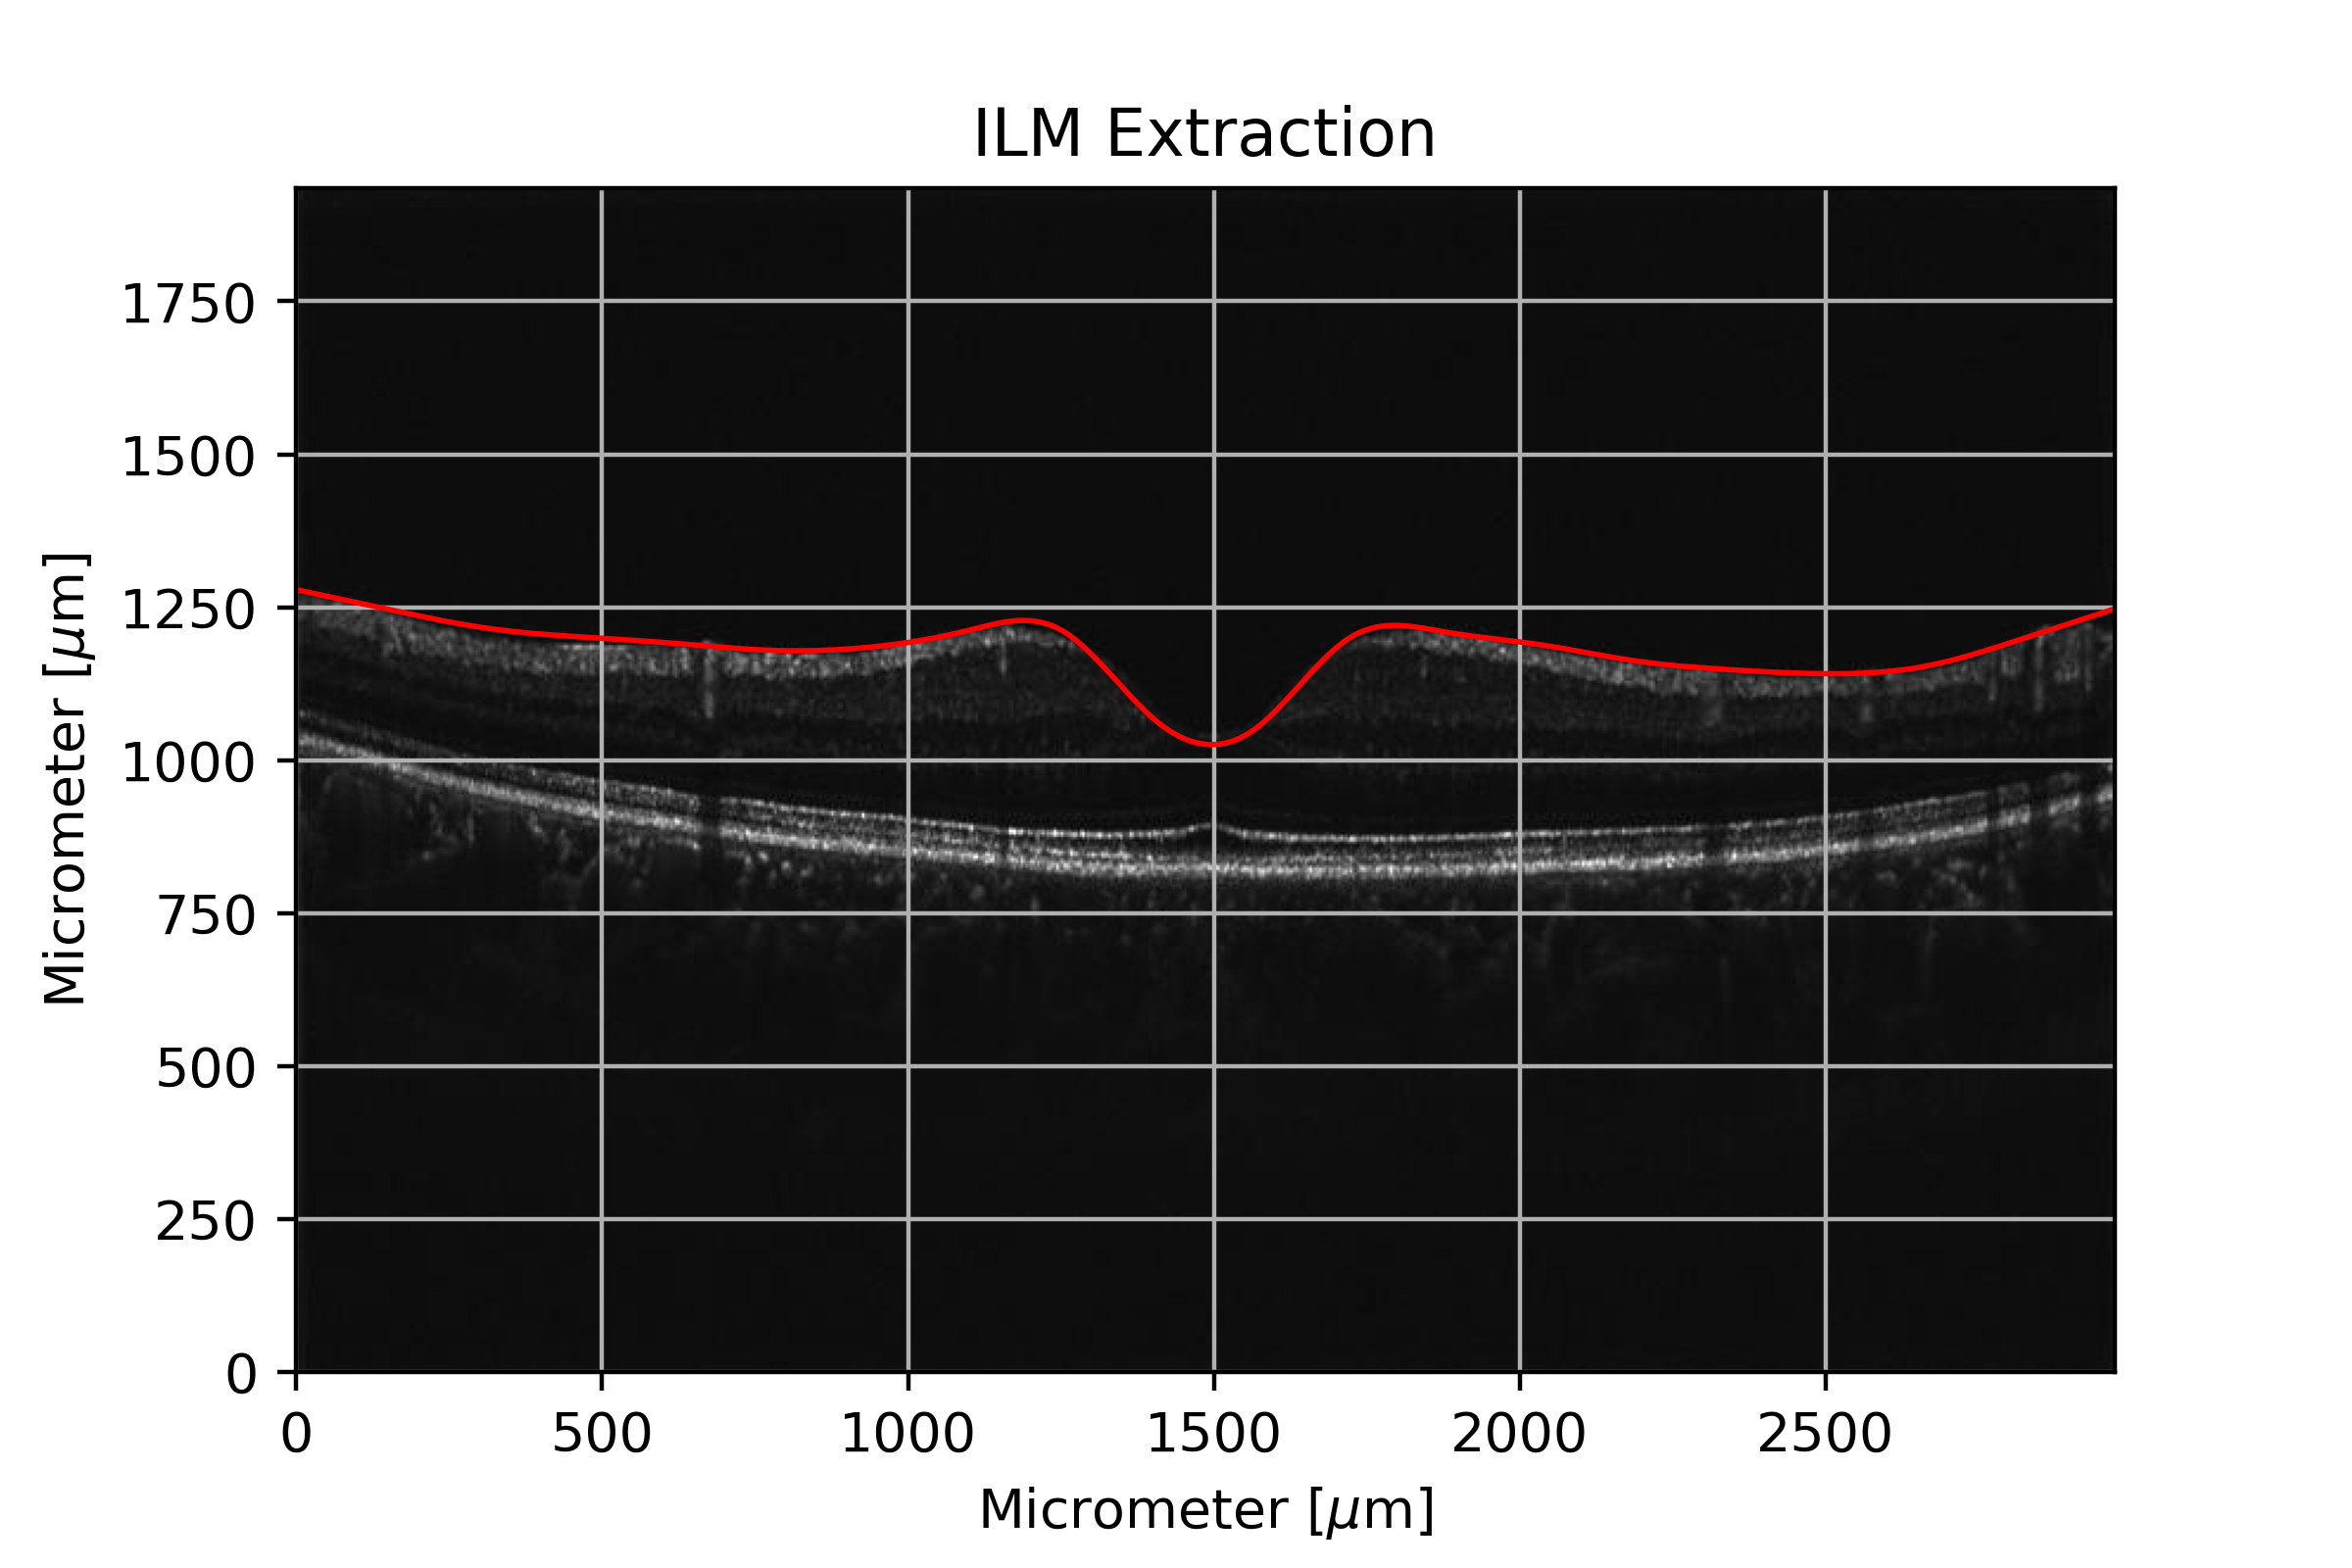
\includegraphics[width=1\textwidth]{./images/ILM_FinalImage.png}
    \caption{ILM extracted}
    \label{fig:ILM_extracted}
\end{figure}



\subsection{BM Extraction}
The procedure for extracting is about the same as for extracting the ILM, however another method has been used to extract the black and white image. While this method was very effective for the detection of ILM, it is less effective for the BM, because the BM is located between the ILM and the choroid. Therefore there's no advantage of having the lens which is rendered black on the scan. Additionally the the BM might be surrounded by other more or less white elements, like the image being treated in this paper. Using the same method as for ILM would make the procedure imprecise.\\
The chosen approach was to extract for the BM was implemented using Python's OpenCV library. OpenCV allows you to extract "lines" according to the lightest parts of the image \cite{stackoverflow:SHEN} \cite{python:opencv}.

\begin{python}
#Here we try to define a more precise line since the retina line extraction have some imperfection
# white color mask
img = cv2.imread('./imageresponse.jpeg')
#converted = convert_hls(img)
image = cv2.cvtColor(img,cv2.COLOR_BGR2HLS)
lower = np.uint8([0, 80, 0])
upper = np.uint8([255, 255, 255])
white_mask = cv2.inRange(image, lower, upper)
# yellow color mask
lower = np.uint8([10, 0,   100])
upper = np.uint8([40, 255, 255])
yellow_mask = cv2.inRange(image, lower, upper)
# combine the mask
mask = cv2.bitwise_or(white_mask, yellow_mask)
result = img.copy()
cv2_imshow(mask)
\end{python}

The result of the black and white mask gives a more precise definition of the BM :
\begin{figure}[H]
    \centering
    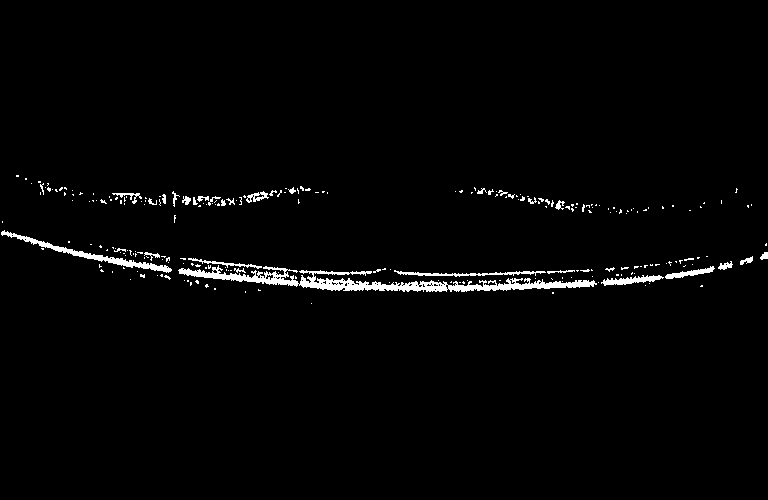
\includegraphics[width=1\textwidth]{./images/Grey_BM.png}
    \caption{BM extraction, black and white mask}
    \label{fig:BM-black_withe}
\end{figure}
Now all that is left to do is to extract a line of pixels as for the ILM. The only difference is that instead of going through the image from top to bottom and extracting the first white pixel encountered, we proceed from bottom to top. The same extreme value processing as for the ILM is applied, this is the exact same process as for the ILM. (section \ref{ILM_Extraction})

Once the natural spline cubic model \cite{stackoverflow:transcranial} is applied \footnote{The softness parameter differs from that of ILM} have obtained the following result  :
\begin{python}
model_10 = get_natural_cubic_spline_model(x, y, minval=min(x), maxval=max(x), n_knots=10)
y_est_10 = model_15.predict(x)
plt.plot(x*micrometerConversion, y_est_10*micrometerConversion,'y', linewidth=1, marker=',', label='n_knots = 10')
\end{python}
\begin{figure}[H]
    \centering
    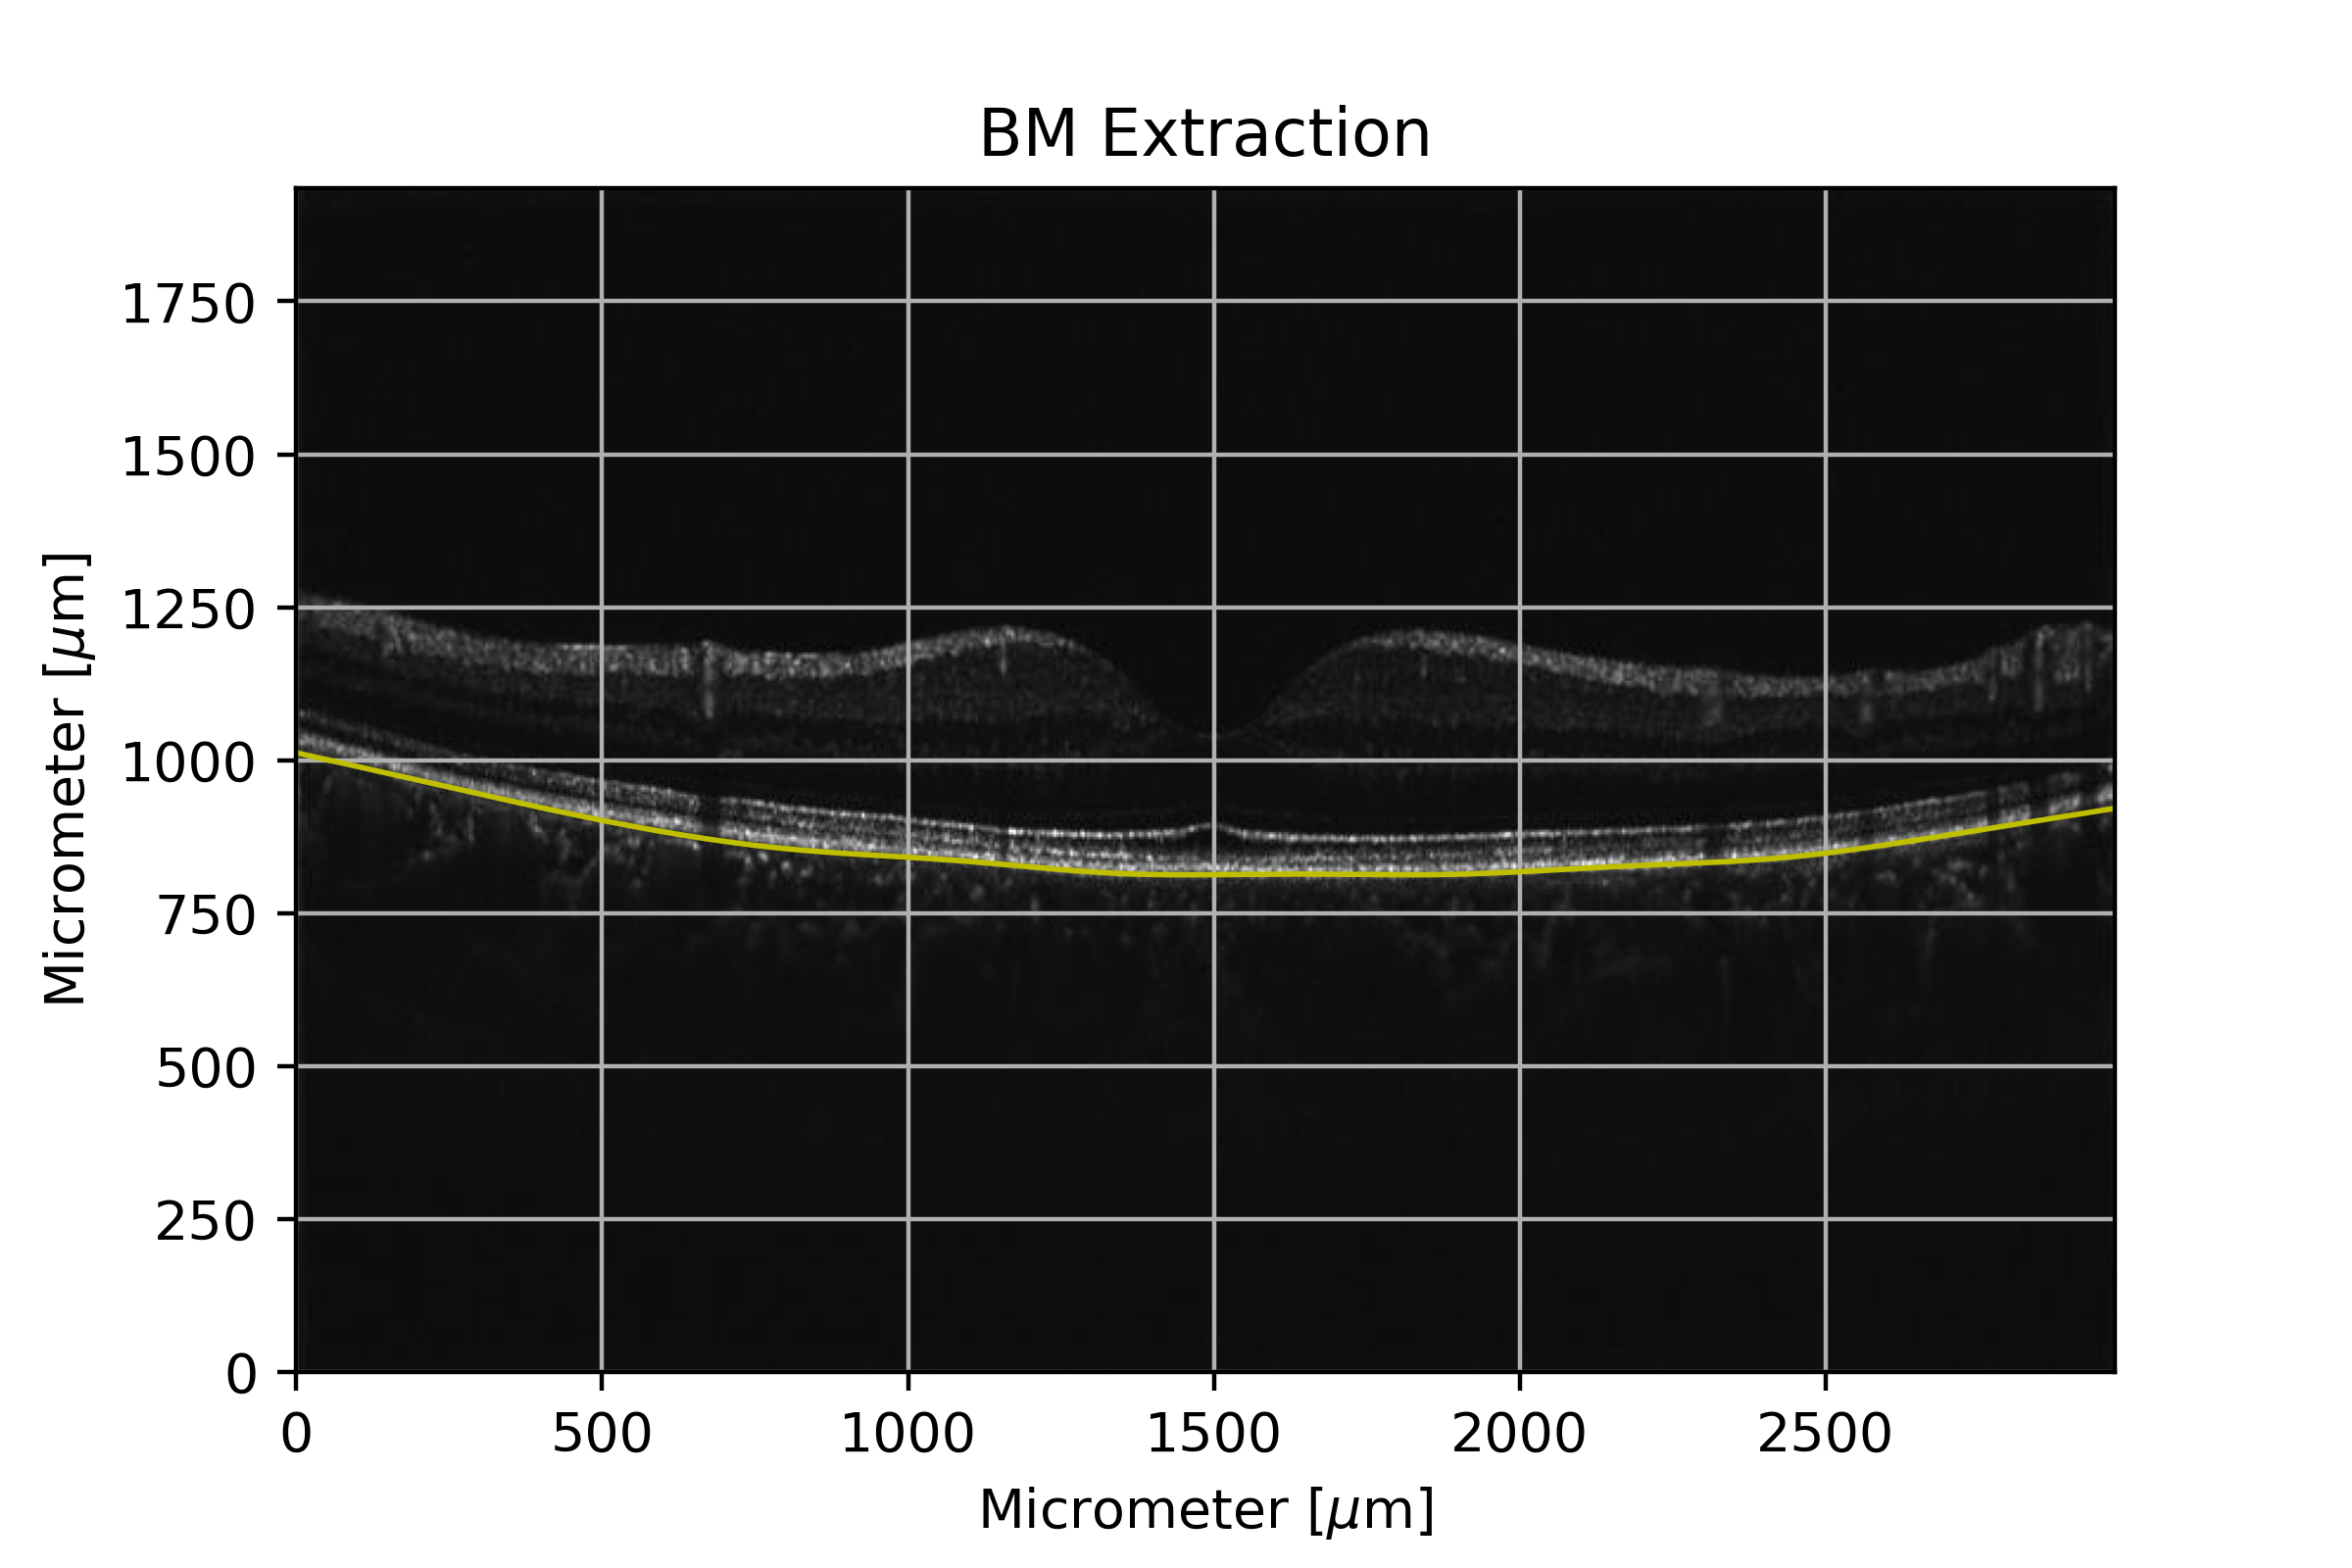
\includegraphics[width=1\textwidth]{./images/BM_FinalImage.png}
    \caption{BM extracted}
    \label{fig:BM-extracted}
\end{figure}

\subsection{Retina's thickness}
As seen in section \ref{TechBack} there are two methods to calculate the retinal thickness.
In order to calculate the average thickness of the retina (method 1), it is sufficient to calculate for each X the distance between the Y points of the ILM and BM curve as follows : 
\begin{figure}[H]
    \centering
    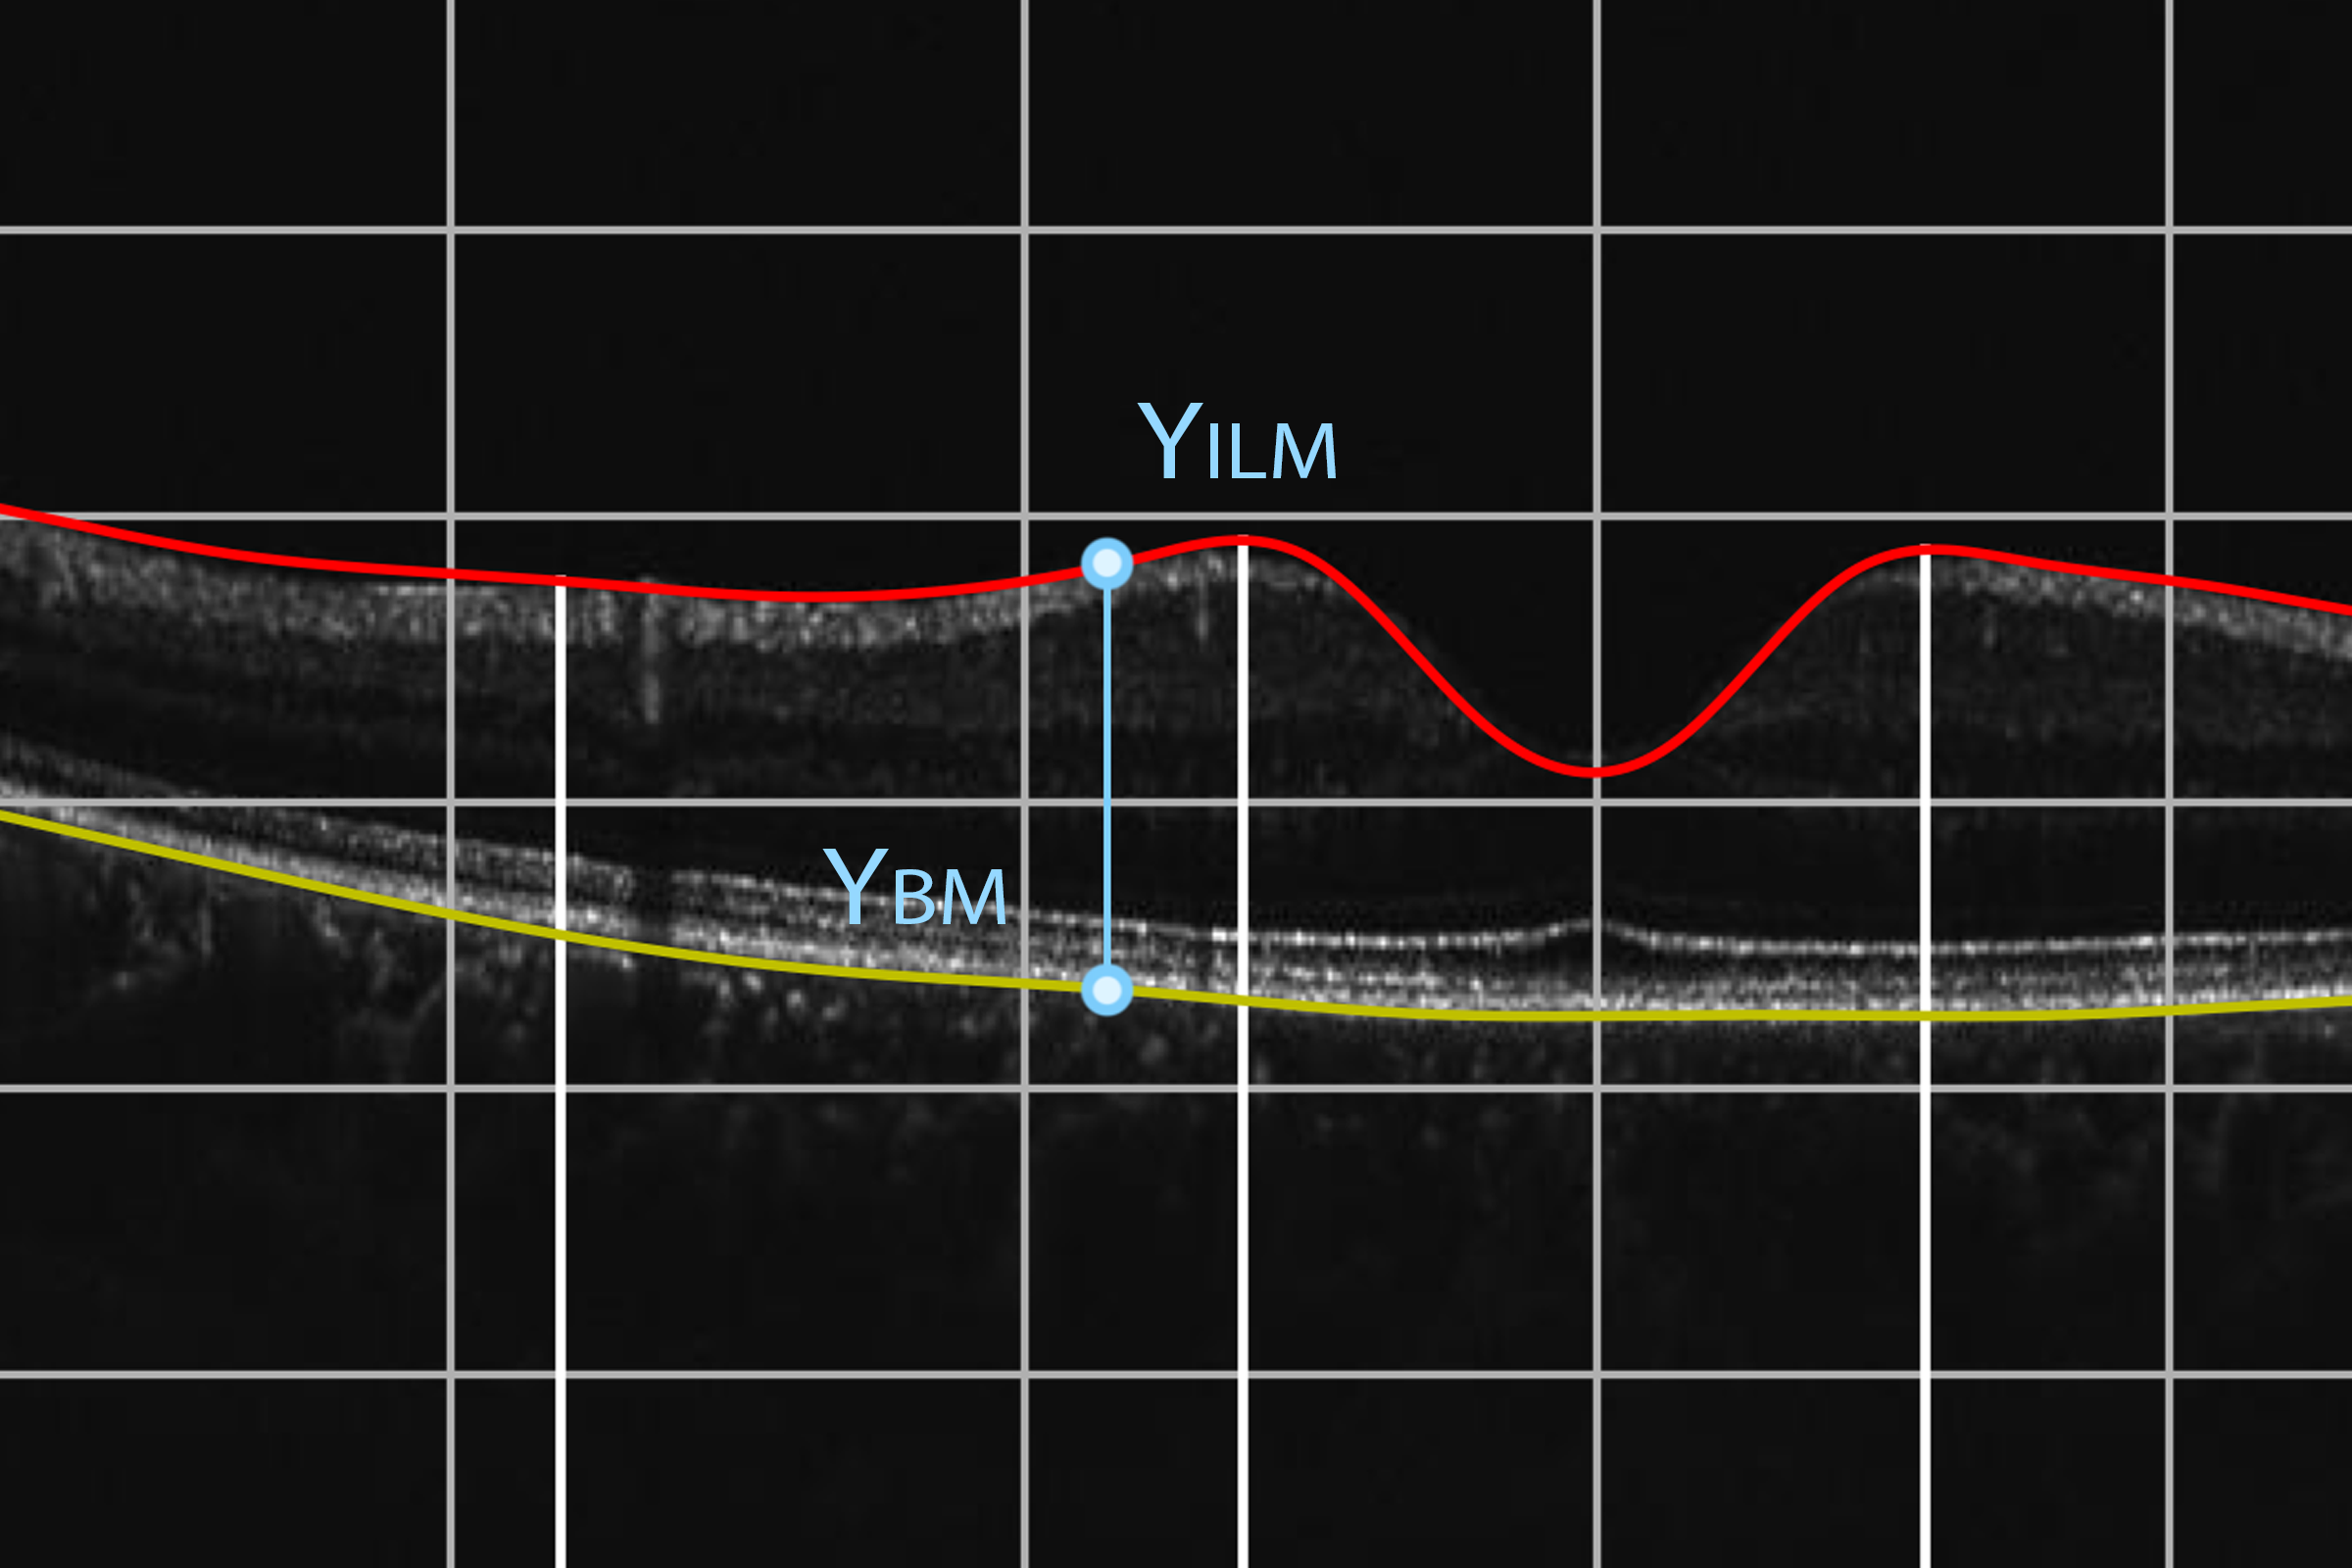
\includegraphics[width=1\textwidth]{./images/ILM_BM_RetinalDistance.png}
    \caption{Retina's thickness on a point X}
    \label{fig:retinat-thickness-x}
\end{figure}
For this, a simple calculation to find the distance between 2 points is necessary. 

\[ distance = \sqrt {\left( {x_{ilm} - x_{bm} } \right)^2 + \left( {y_{ilm} - y_{bm} } \right)^2 } \]
This calculation is applied to all the X points of our graph (\emph{distance} table), it is then sufficient to make a simple average in order to determine the average thickness of the retina (\emph{distanceF}).

\begin{python}
#Retinal thickness Method 1
distance = np.zeros(768, dtype=object)
for i in range(IMG_WIDTH):
  distance[i] =np.sqrt(pow((x_ilm[i] - x_mb[i]), 2) + pow(y_est_35[i] - y_est_10[i], 2))*micrometerConversion
distanceF =  np.around(np.average(distance), decimals=2, out=None)

\end{python}
The 2nd method which consists in separating the scan into 5 sections and calculating the average thickness of each of them, the same calculation is done but the table containing the distances between the ILM and the BM is divided into 5 sections. The \emph{np.array\_split} method allows to separate the distance array into 5 sections, as the size of the stop is 768 px the 5 sections will be separated as follows: 153|153|154|154 px. The difference in section size is minimal and therefore not a problem.
\begin{python}
separatedDistance = np.array_split(distance, 5)
tabSize = 0
sRegions = ['C','B','A','B','C']
for i in range(5):
  placement = np.count_nonzero(separatedDistance[i])
  tabSize += placement
  plt.plot([tabSize*micrometerConversion, tabSize*micrometerConversion], [0, y_est_35[tabSize-1]*micrometerConversion], 'w',linewidth=1)
\end{python}
The final render of the ILM and BM detection to calculate the thickness of the retina looks like this : 
\begin{figure}[H]
    \centering
    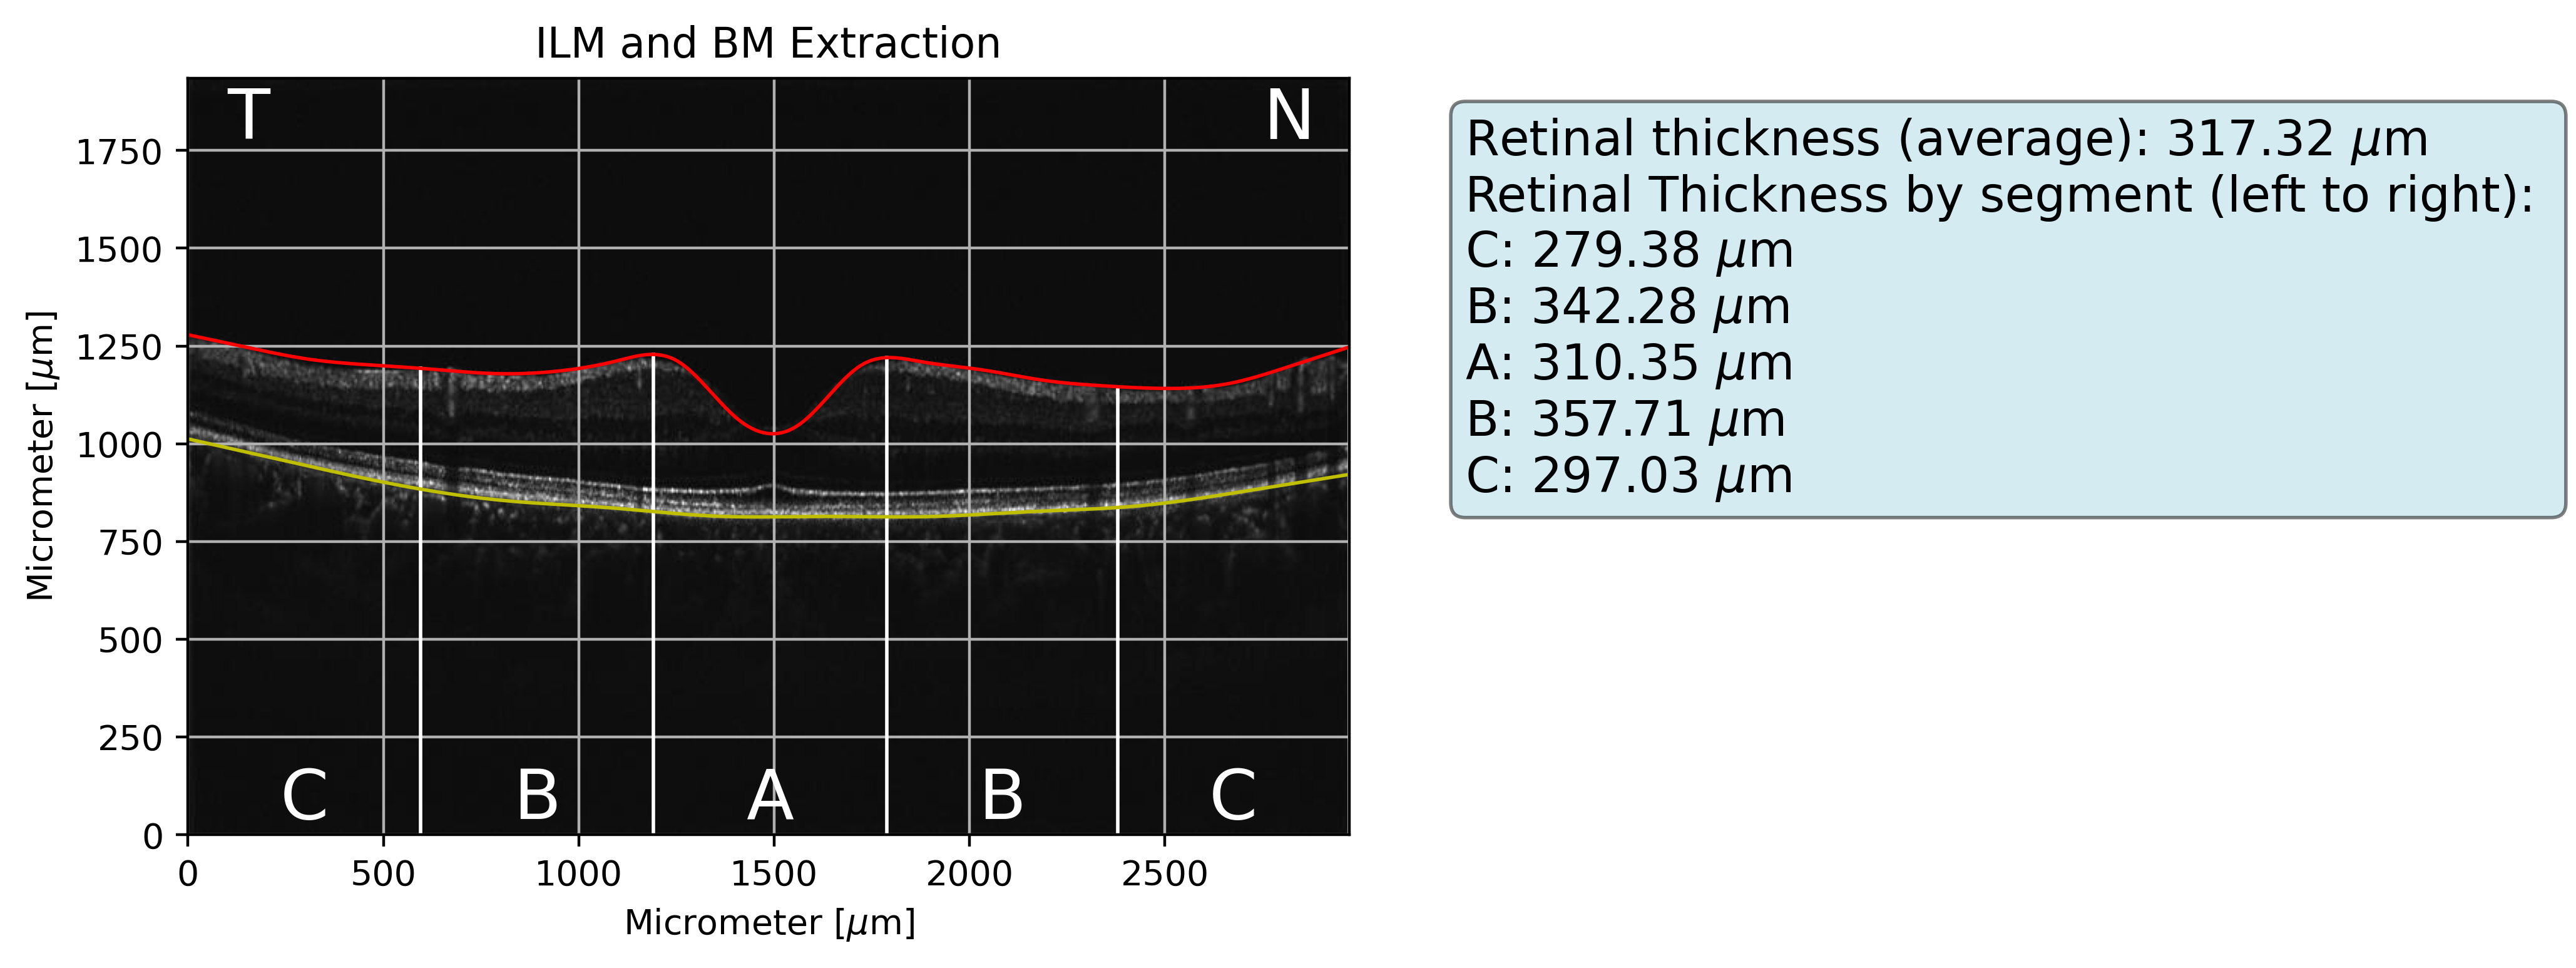
\includegraphics[width=1\textwidth]{./images/ILM_BM_Extracted.png}
    \caption{Final rendering of the ILM, BM and retina thinckness}
    \label{fig:final_rendering}
\end{figure}

\subsection{Limitations Encountered}
Even if this ILM and BM detection solution works well for one scan, it does not mean that it will work optimally for every scan. In the table below 6 different scans have been chosen to see how ILM and BM detection reacts.

\begin{table}[H]
  \centering
  \begin{tabular}{ | m{5cm} | m{5cm} | m{5cm} | }
    \hline
    Base image & Smoothing parameters: ILM : 35, BM : 10 & Smoothing parameter adjusted \\ 
    \hline%B
    \begin{minipage}{.3\textwidth}
      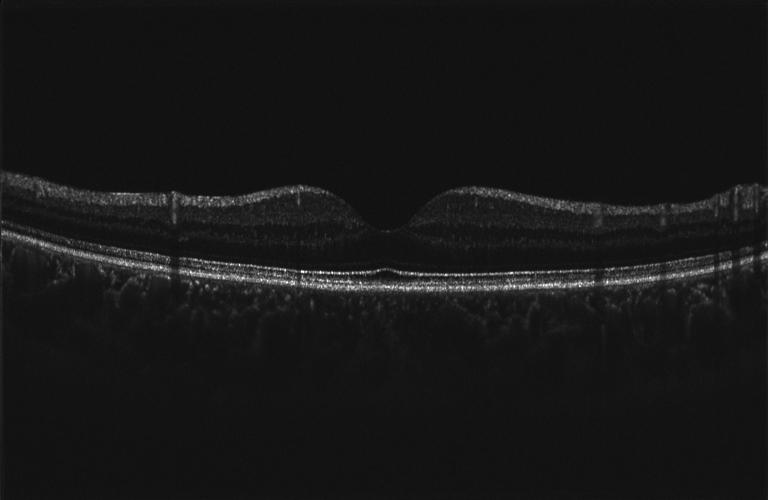
\includegraphics[width=\linewidth]{./images/TableOCT/base1.jpeg}
    \end{minipage}
    &
     \begin{minipage}{.3\textwidth}
      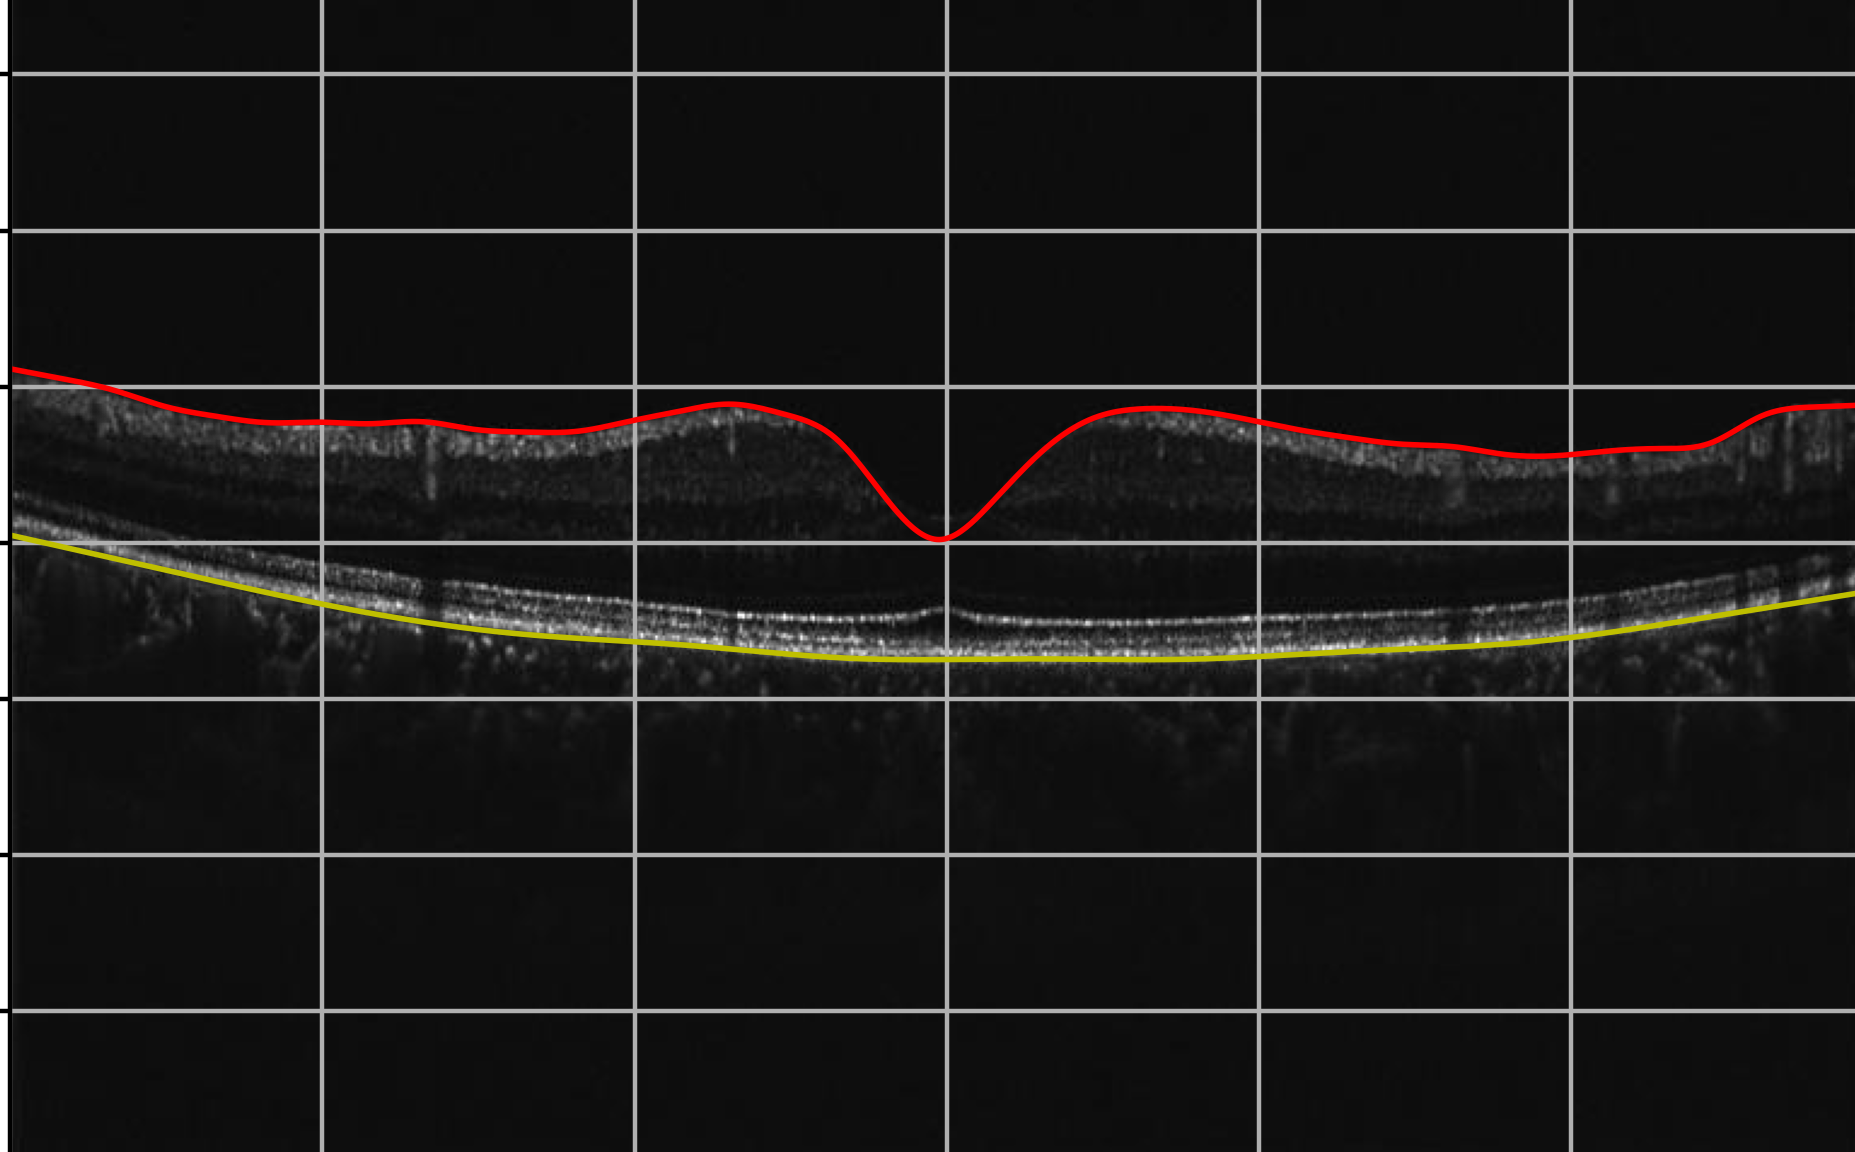
\includegraphics[width=\linewidth]{./images/TableOCT/ILM_BM_1.png}
    \end{minipage}
    & 
     No adjustment needed
    \\ \hline%E
    \begin{minipage}{.3\textwidth}
      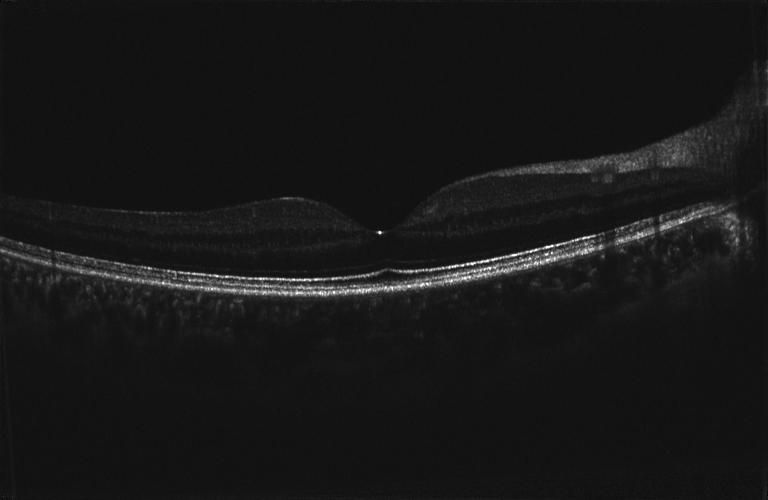
\includegraphics[width=\linewidth]{./images/TableOCT/base2.jpeg}
    \end{minipage}
    &
     \begin{minipage}{.3\textwidth}
      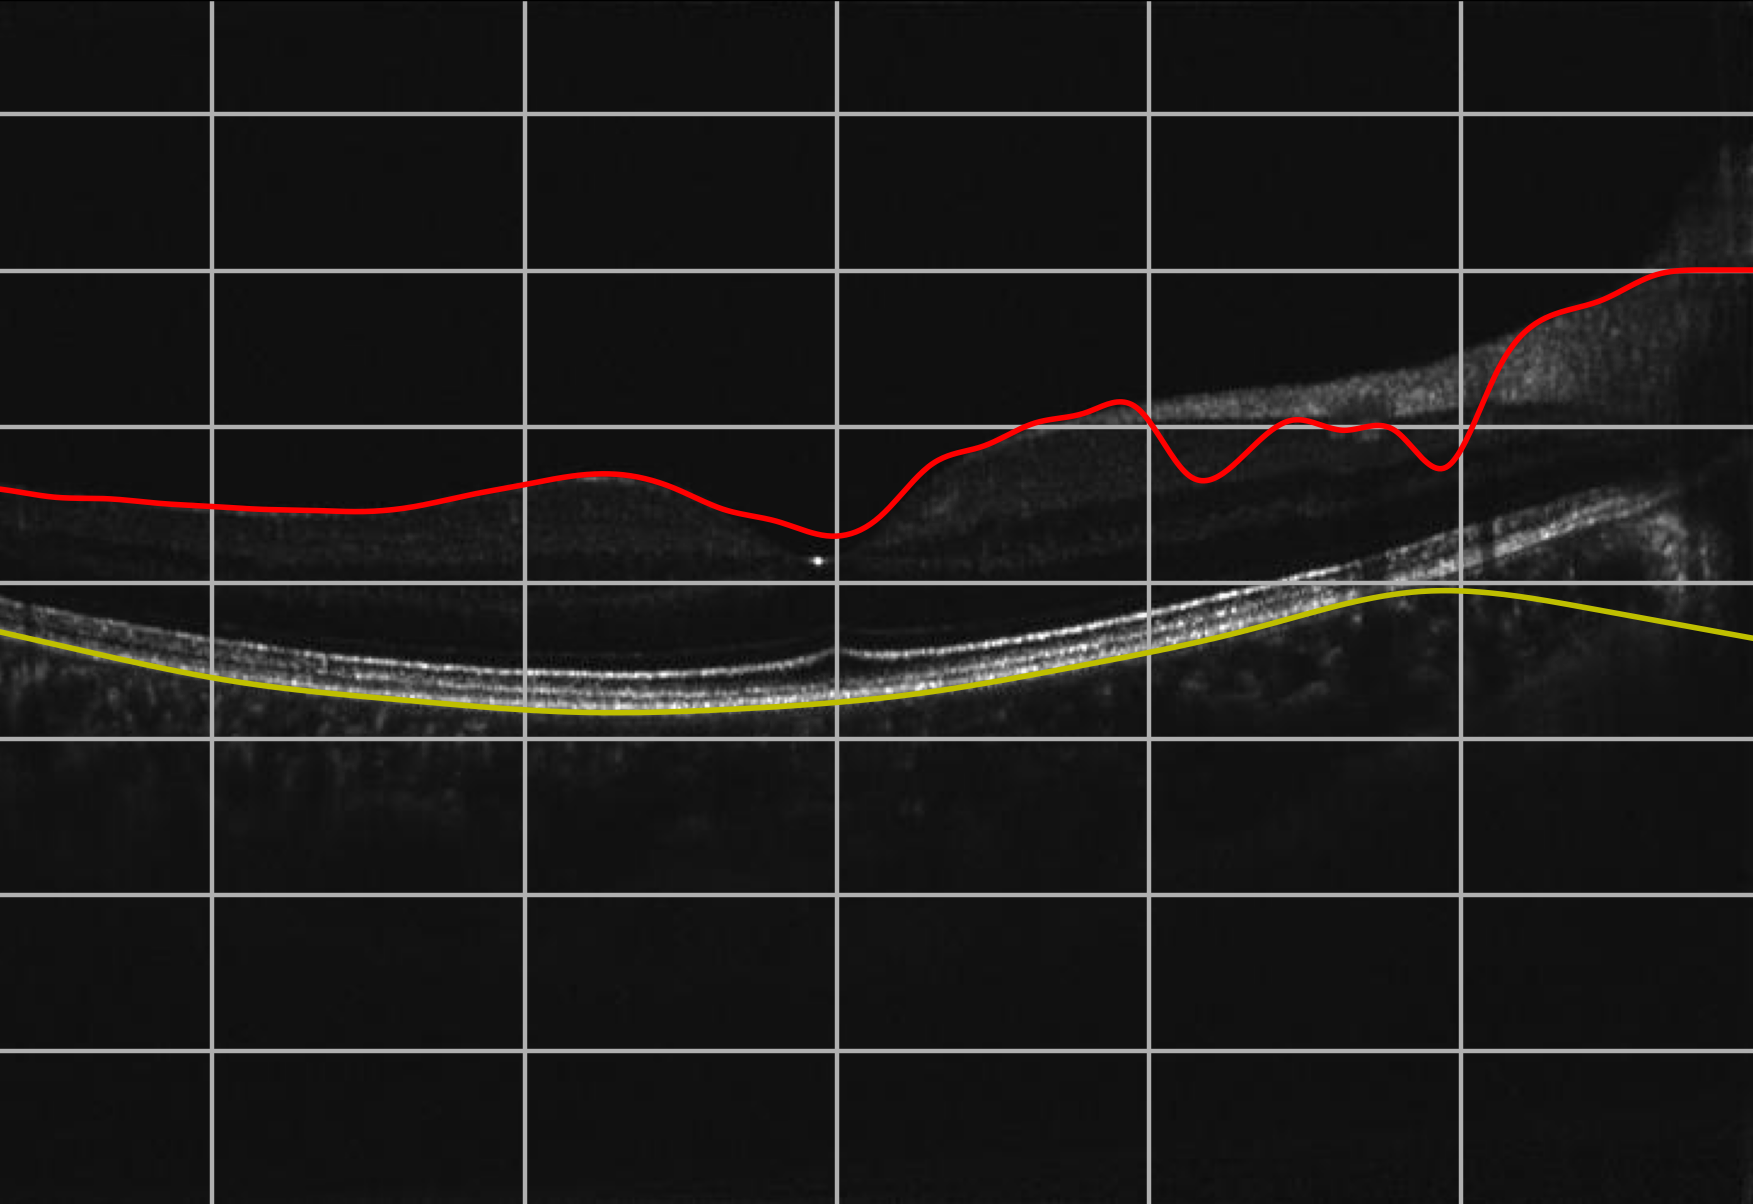
\includegraphics[width=\linewidth]{./images/TableOCT/ILM_BM_2.png}
    \end{minipage}
    & 
     \begin{minipage}{.3\textwidth}
      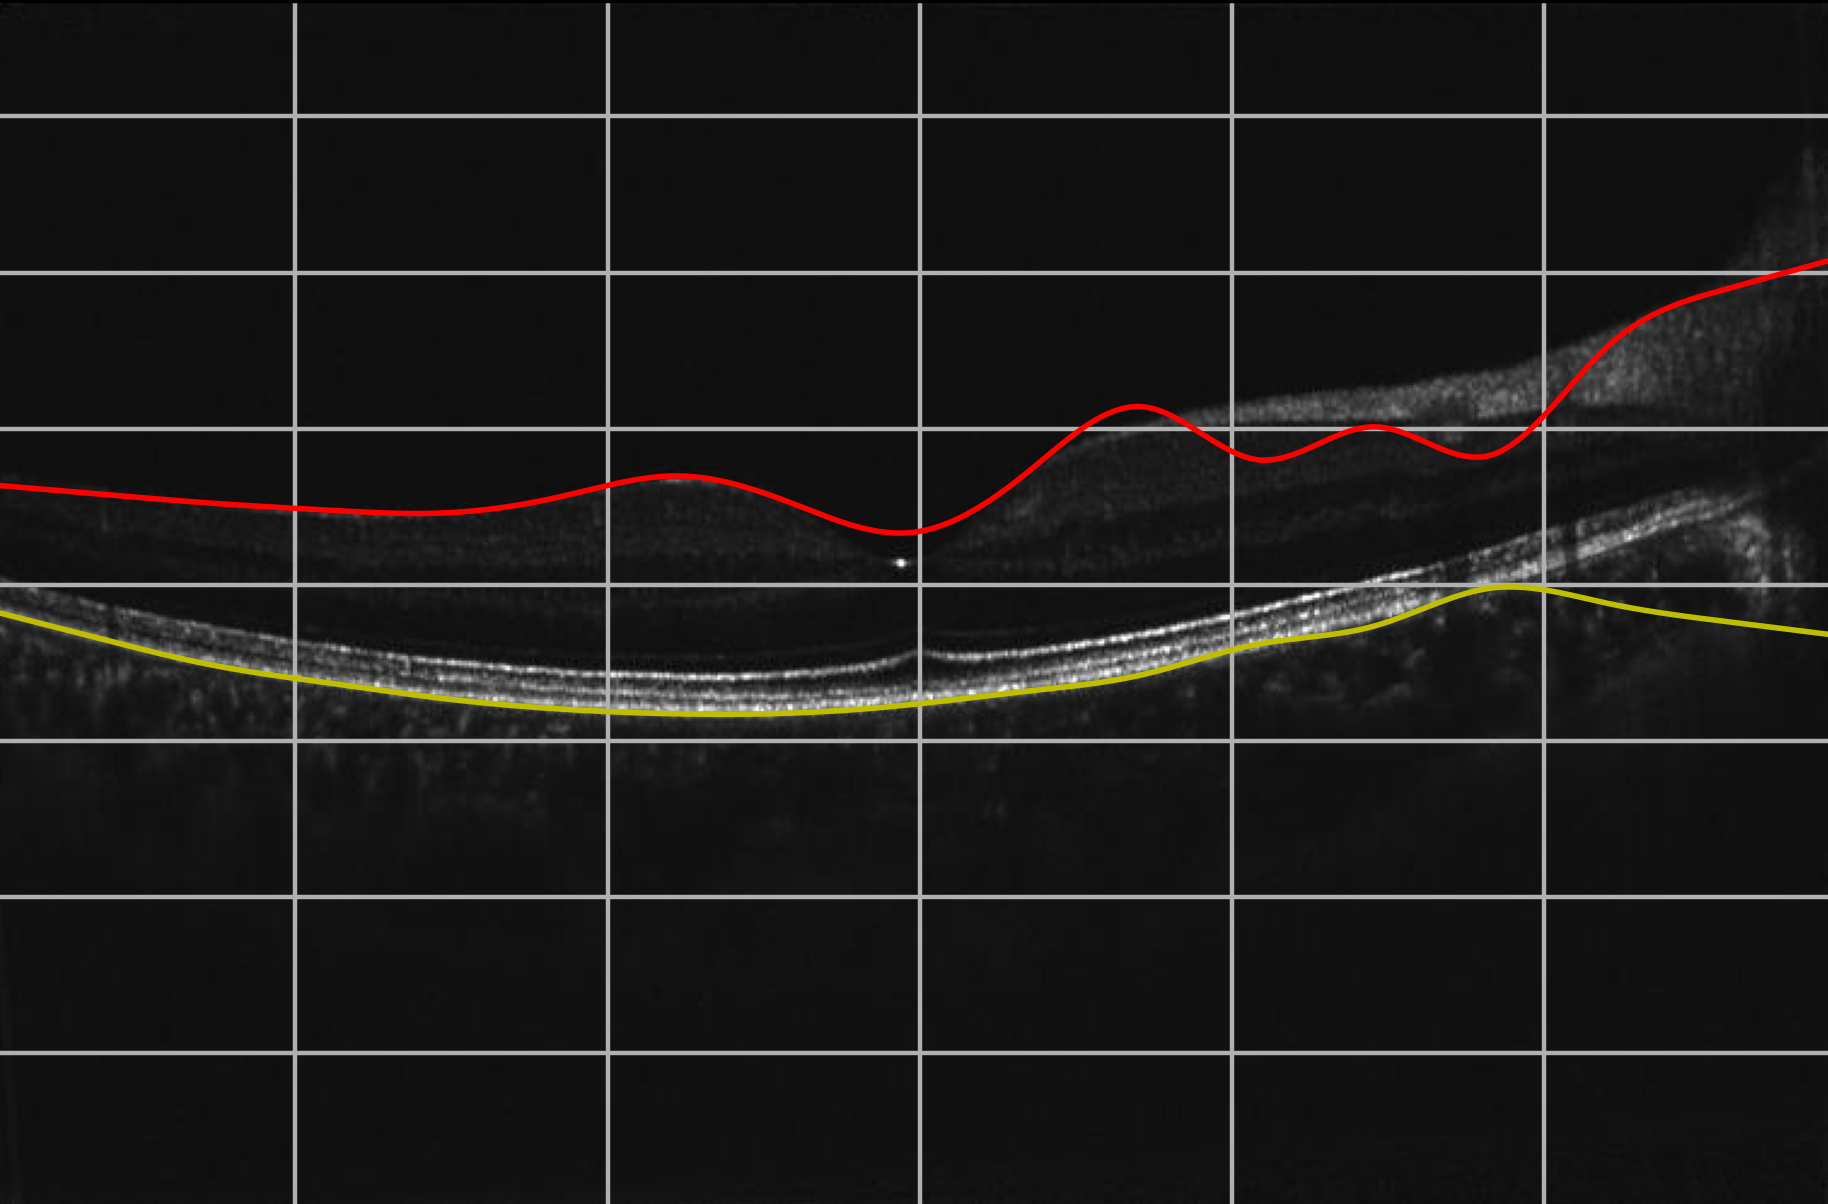
\includegraphics[width=\linewidth]{./images/TableOCT/ILM_BM_2_15_15.png}
    \end{minipage}
    %Smoothing parameters: ILM : 15, BM : 15
    \\ \hline%E
    \begin{minipage}{.3\textwidth}
      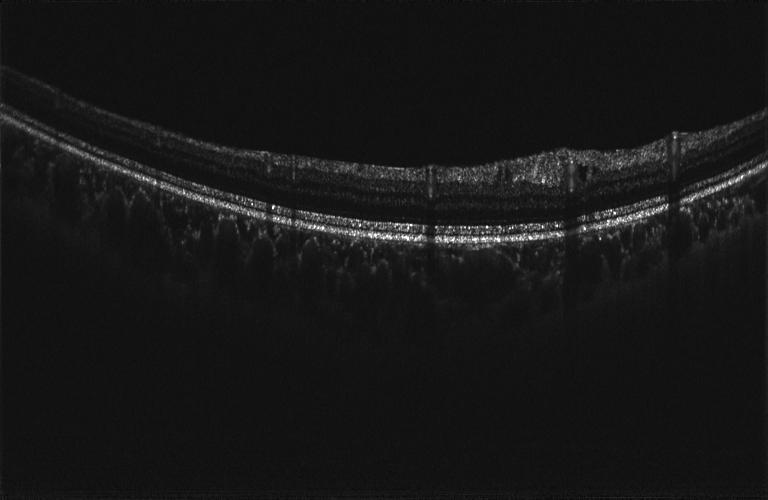
\includegraphics[width=\linewidth]{./images/TableOCT/base3.jpeg}
    \end{minipage}
    &
     \begin{minipage}{.3\textwidth}
      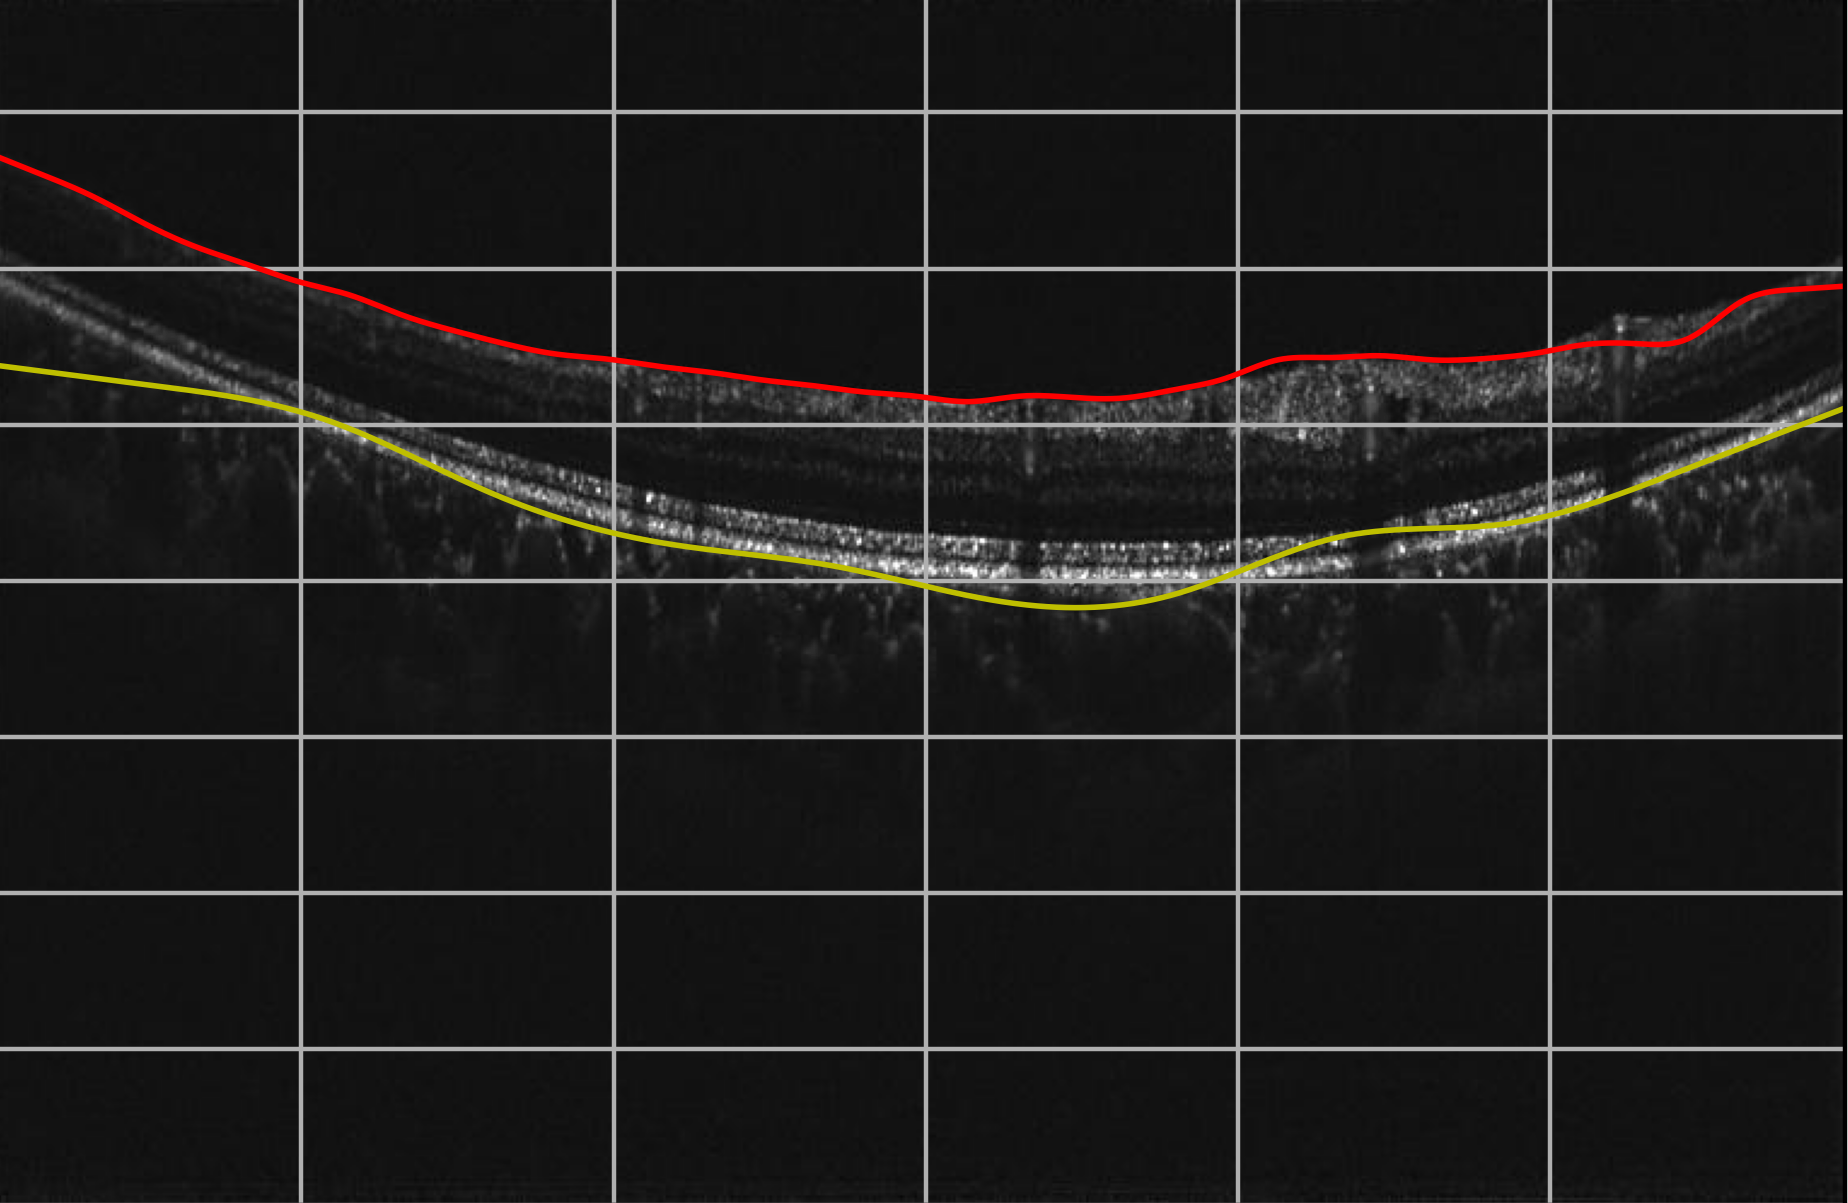
\includegraphics[width=\linewidth]{./images/TableOCT/ILM_BM_3.png}
    \end{minipage}
    & 
     \begin{minipage}{.3\textwidth}
      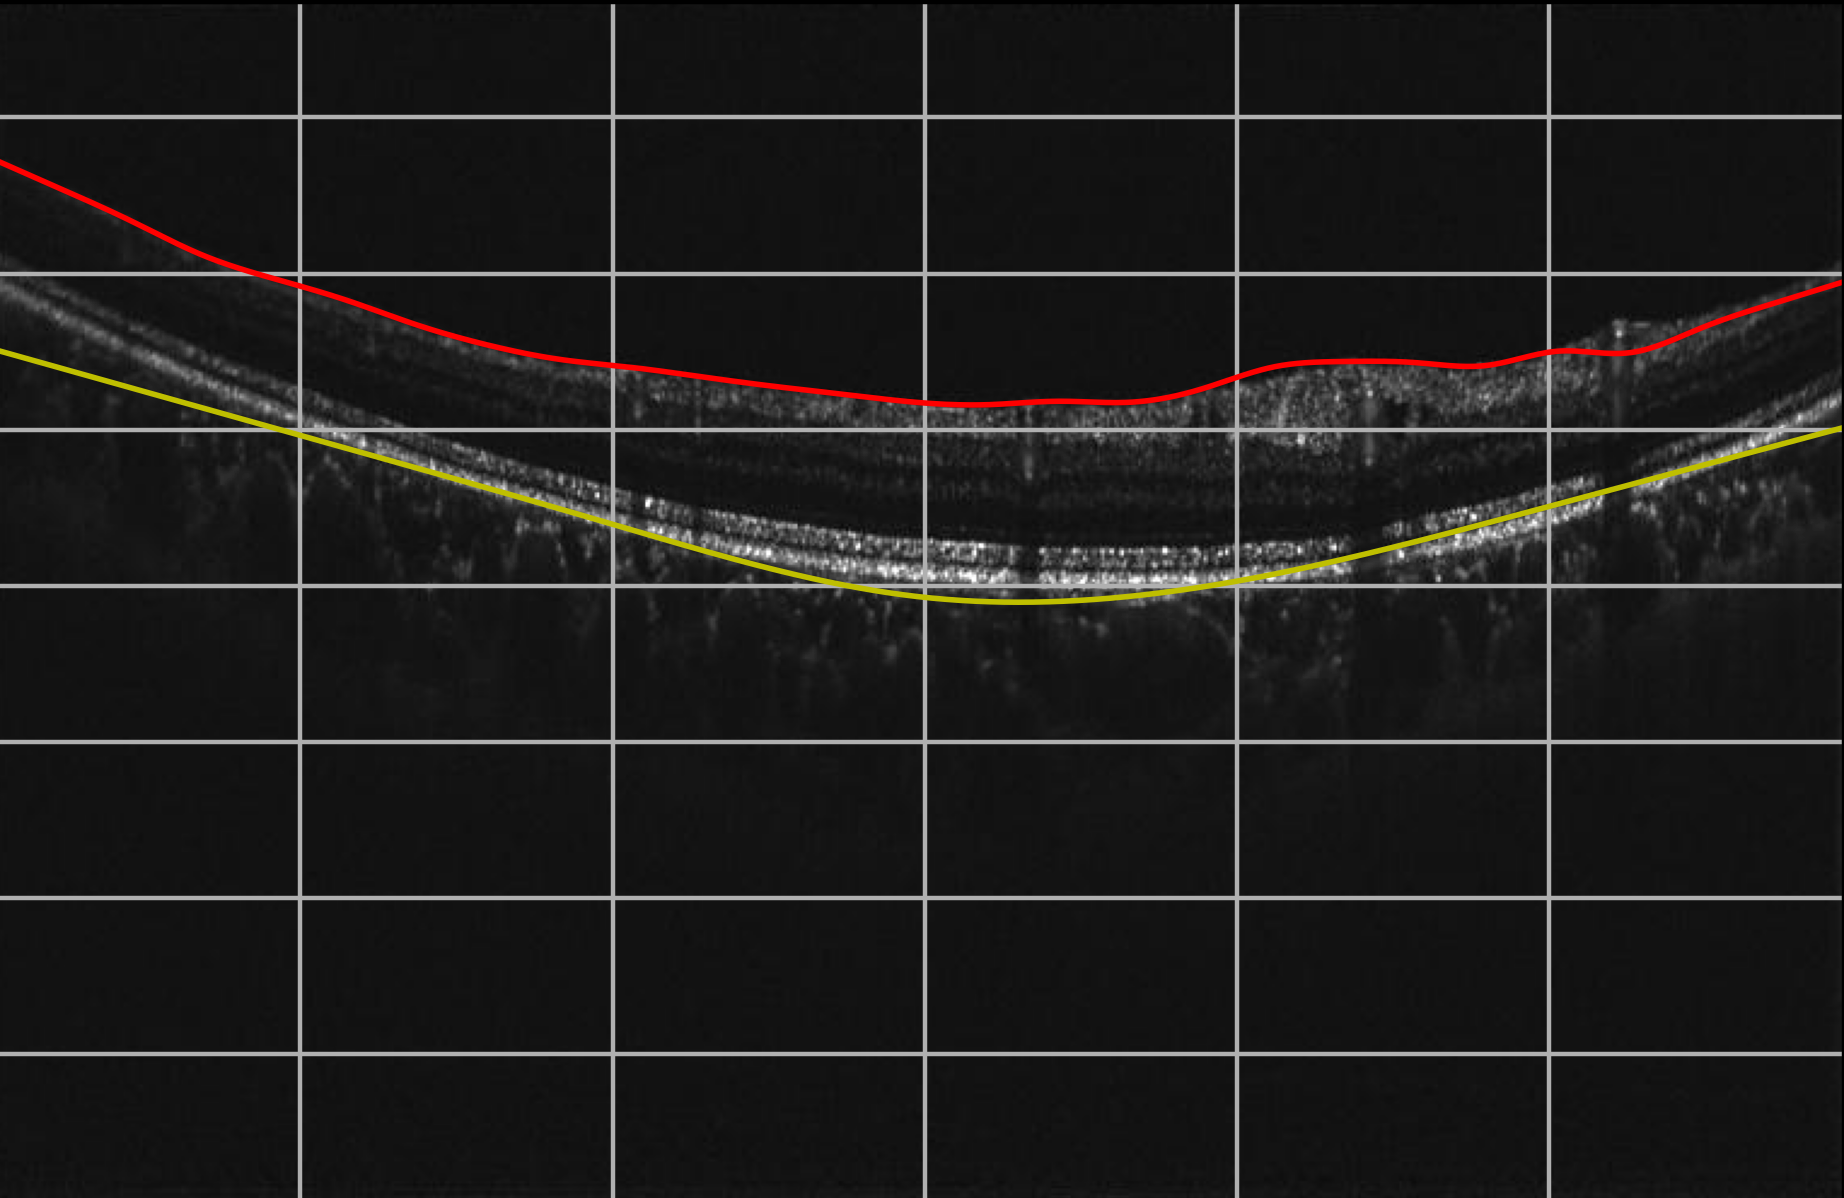
\includegraphics[width=\linewidth]{./images/TableOCT/ILM_BM_3_5_25.png}
    \end{minipage}
    \\ \hline%E
    \begin{minipage}{.3\textwidth}
      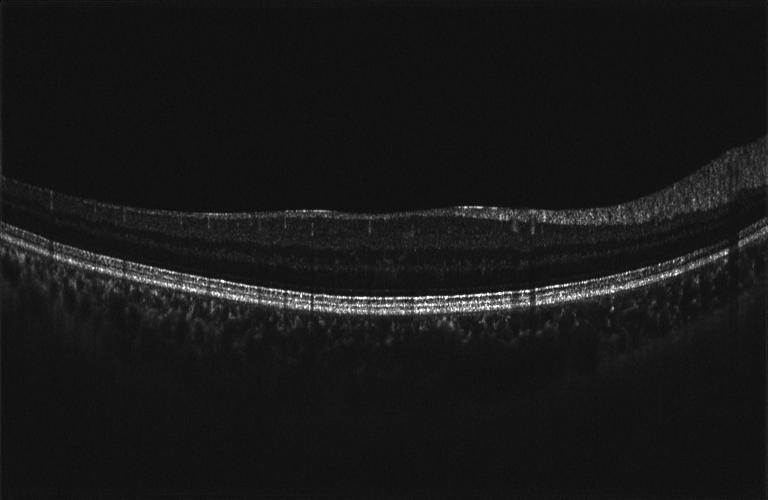
\includegraphics[width=\linewidth]{./images/TableOCT/base4.jpeg}
    \end{minipage}
    &
     \begin{minipage}{.3\textwidth}
      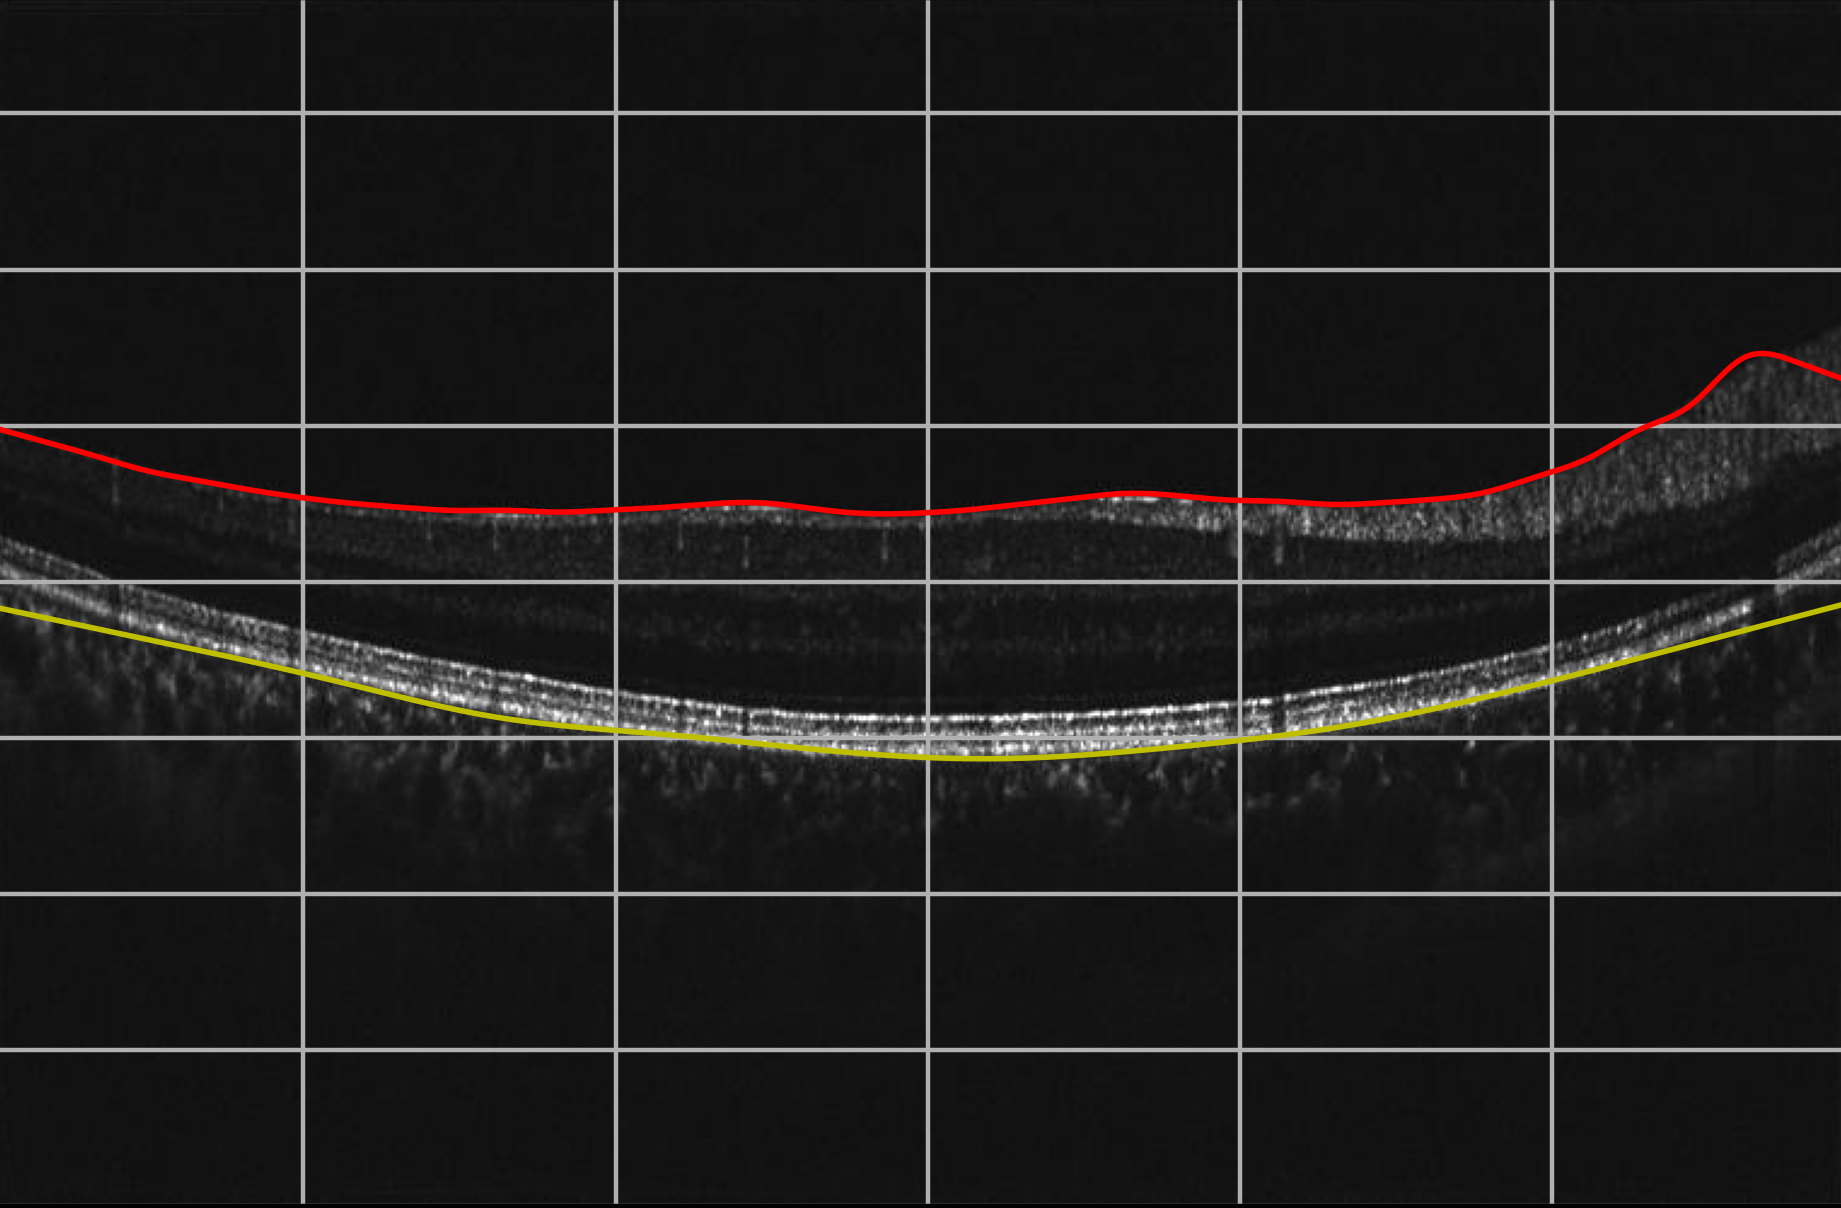
\includegraphics[width=\linewidth]{./images/TableOCT/ILM_BM_4.png}
    \end{minipage}
    & 
    \begin{minipage}{.3\textwidth}
      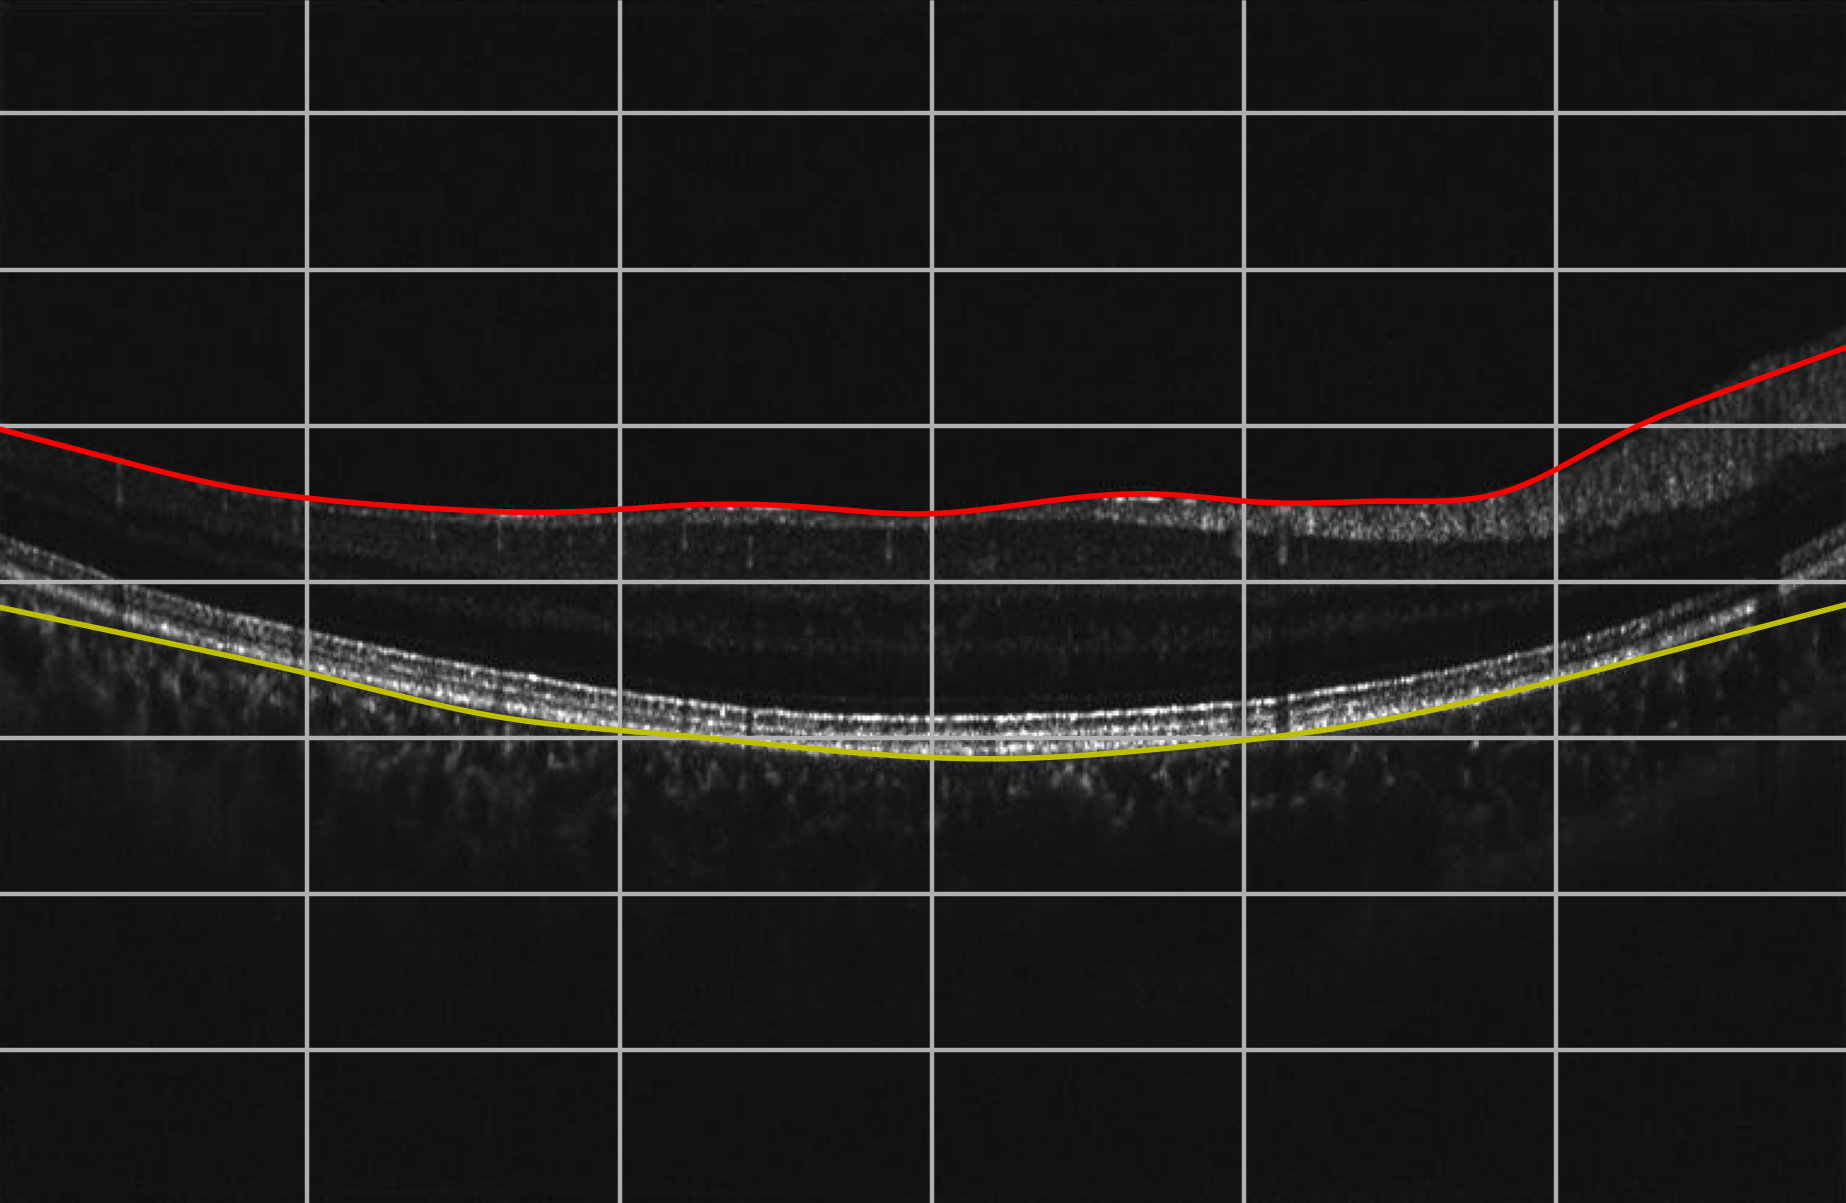
\includegraphics[width=\linewidth]{./images/TableOCT/ILM_BM_4_10_15.png}
    \end{minipage}
    \\ \hline%E
    \begin{minipage}{.3\textwidth}
      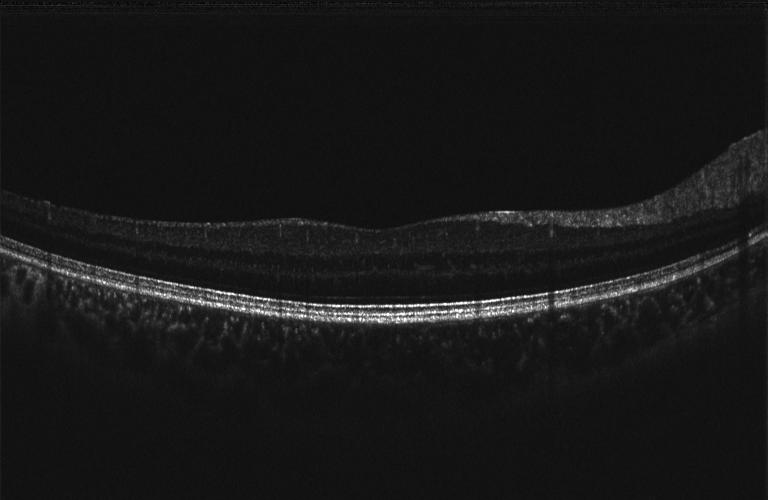
\includegraphics[width=\linewidth]{./images/TableOCT/base5.jpeg}
    \end{minipage}
    &
     \begin{minipage}{.3\textwidth}
      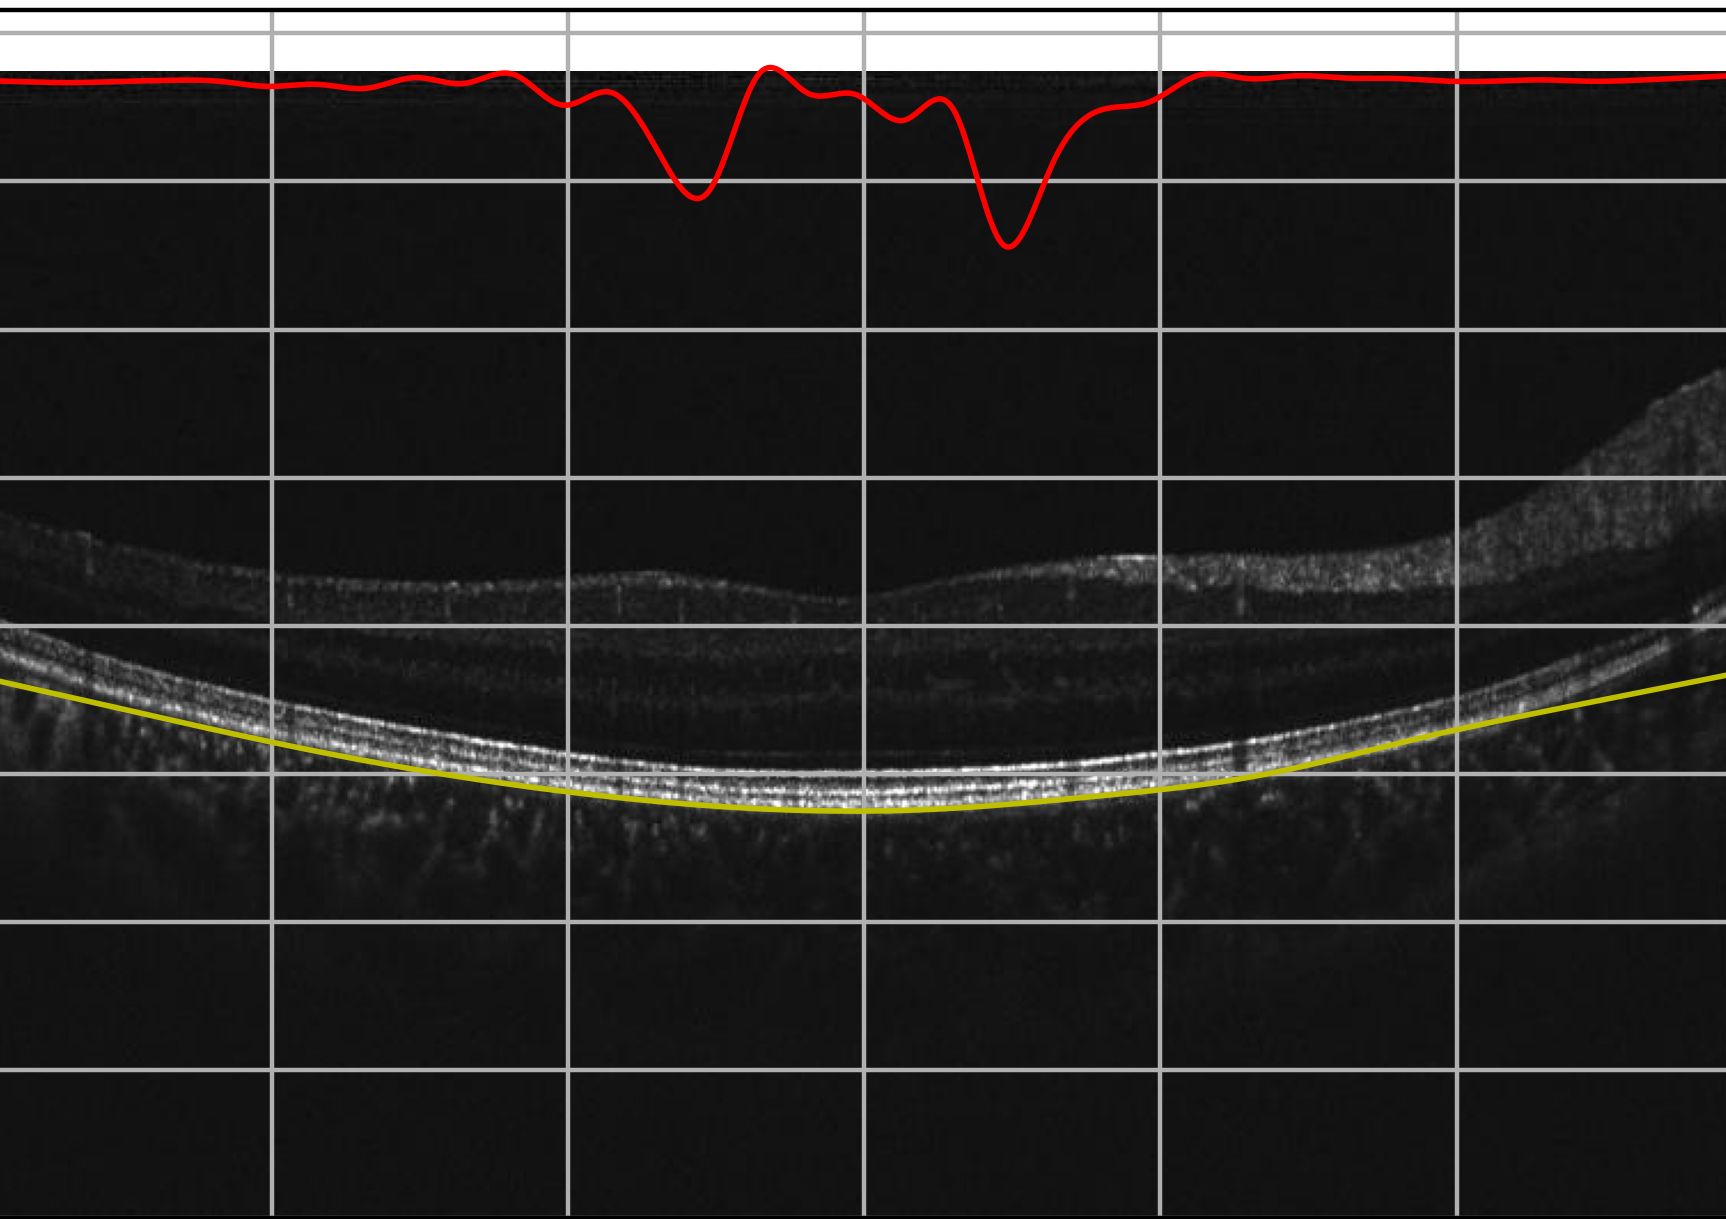
\includegraphics[width=\linewidth]{./images/TableOCT/ILM_BM_5.png}
    \end{minipage}
    & 
     Here  is a good example where the "noise" of the scan was too loud and could not be removed, resulting in the ILM being impossible to identify.
    \\ \hline%E
    \begin{minipage}{.3\textwidth}
      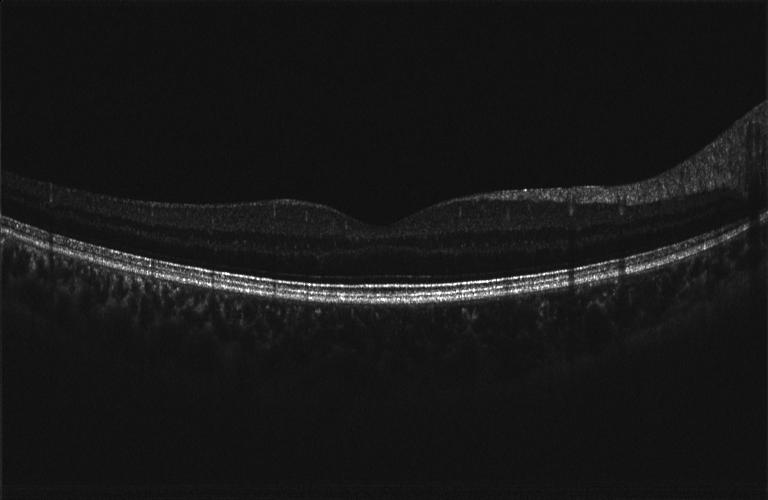
\includegraphics[width=\linewidth]{./images/TableOCT/base6.jpeg}
    \end{minipage}
    &
     \begin{minipage}{.3\textwidth}
      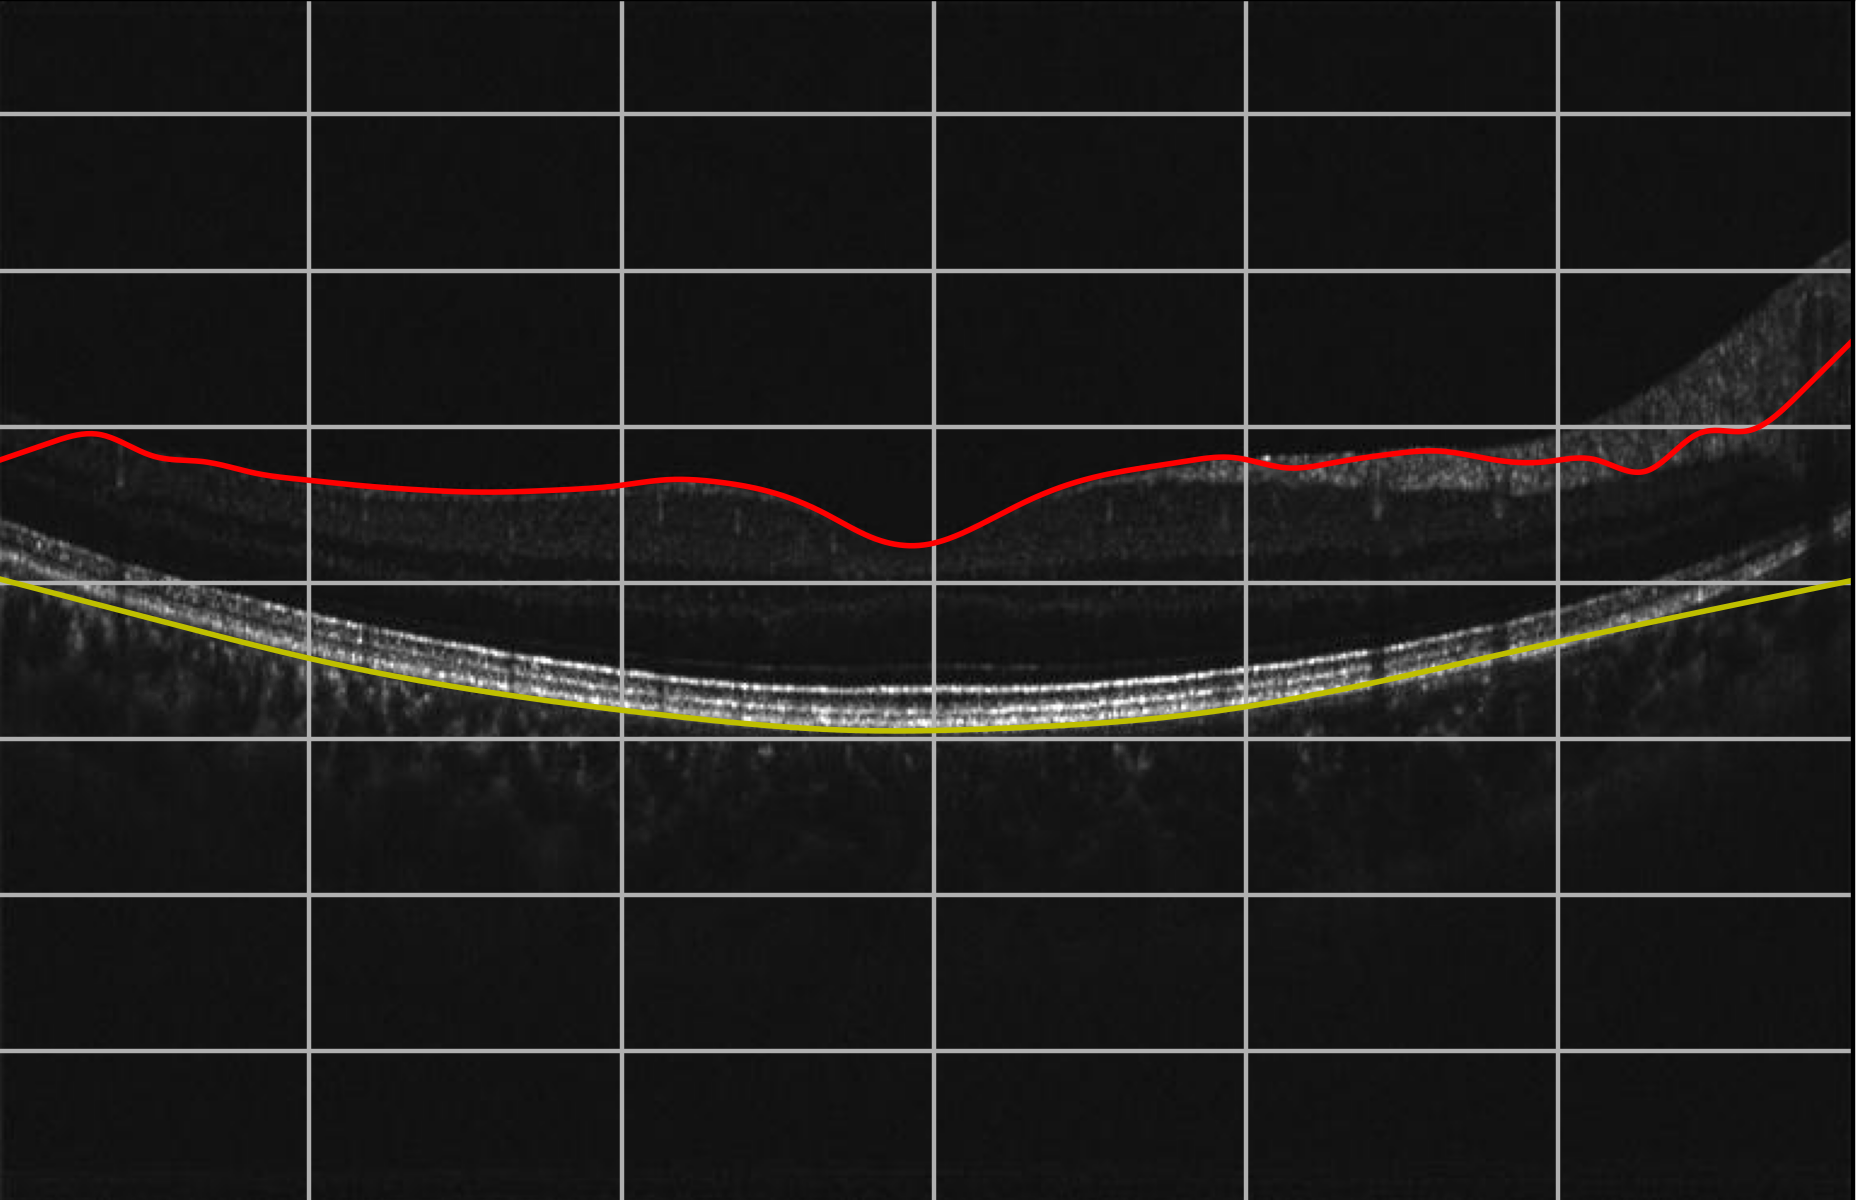
\includegraphics[width=\linewidth]{./images/TableOCT/ILM_BM_6.png}
    \end{minipage}
    & 
     Here we can see that it is not precise on the left, but the rest is good. No adjustment could fix it.
    \\ \hline%E
  \end{tabular}
  \caption{Analysis of the result of several retinal boundaries detection tasks from different OCT scans}\label{tbl:analysis}
\end{table}


The key takeaway from these tests is that the success of the detection algorithm depends very much on the basic quality of the OCT scan. The success of BM and especially ILM identification is not guaranteed every time when working with pixel intensity variations, however, as can be seen in the third column of Table \ref{tbl:analysis}, adjusting the natural smoothing spline parameter can improve the accuracy of ILM and BM detection in certain cases. 

One solution could be to develop a graphical user interface to load OCT scans, detect ILM and BM, and add a user-configurable parameters to manage the natural smoothing spline in order to manually determine the best parameter for each scan.


\section{Conclusion}
\section{Future Work}
As the first step of our investigation, we have decided to algorithmically detect the retinal boundaries in order to give a mean value for its thickness measurement, this process can be error prone considering that a variation in intensity of the B-Scan pixels can introduce artifacts that would create irregularities on the final output. Therefore this controlled implementation will serve us as a base in order to annotate OCT scans and build a deep learning model that can perform the task of recognizing retinal boundaries on a more efficient way across a higher number and varieties of scans allowing for a more flexible boundary detection. The model can be extended to detect the Choroid-Sclera Interface (CSI) potentially allowing to automate the choroid thickness measuring process, but it is important to take into consideration the lack of available experts in order to annotate the scans and the fact that it has been demonstrated that experts present inconsistencies when detecting the CSI even among identical images \cite{Ronchetti2019statistic} which may introduce biases in the deep learning model. Therefore a previous evaluation of the feasibility of the project is to be undertaken.   

\markboth{}{}

\newpage

\bibliographystyle{plain} % We choose the "plain" reference style
\bibliography{bibli} % Entries are in the "bibi.bib" file




\newpage
\thispagestyle{empty}
\markboth{}{}
  \normalsize
\begin{center}
\huge{\textbf{ Declaration of Independence}}\\[40mm]
\end{center}
\large
I affirm that the above work has been produced by myself without any unauthorized assistance and without the use of any other means than those indicated, and that I have marked as such all passages that have been taken literally or meaningfully from published or unpublished writings.\\[50mm]
Bienne, the \today

\newpage



\end{document}